

%----------------------------------------------------------------------------------------
%	PACKAGES AND OTHER DOCUMENT CONFIGURATIONS
%----------------------------------------------------------------------------------------

\documentclass[11pt,fleqn]{book}
% Default font size and left-justified equations
\usepackage{listings}
\usepackage{mdframed}
\usepackage{enumitem}
\usepackage{pifont}
\usepackage{mathtools}
\usepackage{verbatim} 
\DeclarePairedDelimiter{\ceil}{\lceil}{\rceil} 
\DeclarePairedDelimiter{\floor}{\lfloor}{\rfloor}

\newcommand{\pitem}[1]{\item {\small #1}}
\usepackage{algorithm}
\usepackage{algorithmic}
\usepackage{tikz-qtree}
\lstset{language=C++,
    frame=tb, % draw a frame at the top and bottom of the code block
    tabsize=4, % tab space width
    showstringspaces=false, % don't mark spaces in strings
    numbers=left, % display line numbers on the left
    commentstyle=\color{orange}, % comment color
    keywordstyle=\color{blue}, % keyword color
    stringstyle=\color{red} % string color
}
%----------------------------------------------------------------------------------------

%%%%%%%%%%%%%%%%%%%%%%%%%%%%%%%%%%%%%%%%%
% The Legrand Orange Book
% Structural Definitions File
% Version 2.0 (9/2/15)
%
% Original author:
% Mathias Legrand (legrand.mathias@gmail.com) with modifications by:
% Vel (vel@latextemplates.com)
% 
% This file has been downloaded from:
% http://www.LaTeXTemplates.com
%
% License:
% CC BY-NC-SA 3.0 (http://creativecommons.org/licenses/by-nc-sa/3.0/)
%
%%%%%%%%%%%%%%%%%%%%%%%%%%%%%%%%%%%%%%%%%

%----------------------------------------------------------------------------------------
%	VARIOUS REQUIRED PACKAGES AND CONFIGURATIONS
%----------------------------------------------------------------------------------------

\usepackage[top=3cm,bottom=3cm,left=3cm,right=3cm,headsep=10pt,a4paper]{geometry} % Page margins

\usepackage{graphicx} % Required for including pictures
\graphicspath{{Pictures/}} % Specifies the directory where pictures are stored

\usepackage{lipsum} % Inserts dummy text
\usepackage{tikz} % Required for drawing custom shapes
\usepackage{pgfplots}
\pgfplotsset{width=10cm,compat=1.9}
\usepackage[english]{babel} % English language/hyphenation
\usepackage{lettrine}
\usepackage{enumitem} % Customize lists
\setlist{nolistsep} % Reduce spacing between bullet points and numbered lists
%\usepackage{charter}
\usepackage{booktabs} % Required for nicer horizontal rules in tables

\usepackage{xcolor} % Required for specifying colors by name
\definecolor{ocre}{RGB}{243,102,25} % Define the orange color used for highlighting throughout the book

%----------------------------------------------------------------------------------------
%	FONTS
%----------------------------------------------------------------------------------------

\usepackage{avant} % Use the Avantgarde font for headings
%\usepackage{times} % Use the Times font for headings
\usepackage{mathptmx} % Use the Adobe Times Roman as the default text font together with math symbols from the Sym­bol, Chancery and Com­puter Modern fonts

\usepackage{microtype} % Slightly tweak font spacing for aesthetics
\usepackage[utf8]{inputenc} % Required for including letters with accents
\usepackage[T1]{fontenc} % Use 8-bit encoding that has 256 glyphs

%----------------------------------------------------------------------------------------
%	BIBLIOGRAPHY AND INDEX
%----------------------------------------------------------------------------------------

\usepackage{csquotes}
\usepackage[style=alphabetic,citestyle=numeric,sorting=nyt,sortcites=true,autopunct=true,autolang=hyphen,hyperref=true,abbreviate=false,backref=true,backend=biber,defernumbers=true]{biblatex}
\addbibresource{bibliography.bib} % BibTeX bibliography file
\defbibheading{bibempty}{}

\usepackage{calc} % For simpler calculation - used for spacing the index letter headings correctly
\usepackage{makeidx} % Required to make an index
\makeindex % Tells LaTeX to create the files required for indexing

%----------------------------------------------------------------------------------------
%	MAIN TABLE OF CONTENTS
%----------------------------------------------------------------------------------------

\usepackage{titletoc} % Required for manipulating the table of contents

\contentsmargin{0cm} % Removes the default margin

% Part text styling
\titlecontents{part}[0cm]
{\addvspace{20pt}\centering\large\bfseries}
{}
{}
{}

% Chapter text styling
\titlecontents{chapter}[1.25cm] % Indentation
{\addvspace{12pt}\large\sffamily\bfseries} % Spacing and font options for chapters
{\color{ocre!60}\contentslabel[\Large\thecontentslabel]{1.25cm}\color{ocre}} % Chapter number
{\color{ocre}}  
{\color{ocre!60}\normalsize\;\titlerule*[.5pc]{.}\;\thecontentspage} % Page number

% Section text styling
\titlecontents{section}[1.25cm] % Indentation
{\addvspace{3pt}\sffamily\bfseries} % Spacing and font options for sections
{\contentslabel[\thecontentslabel]{1.25cm}} % Section number
{}
{\hfill\color{black}\thecontentspage} % Page number
[]

% Subsection text styling
\titlecontents{subsection}[1.25cm] % Indentation
{\addvspace{1pt}\sffamily\small} % Spacing and font options for subsections
{\contentslabel[\thecontentslabel]{1.25cm}} % Subsection number
{}
{\ \titlerule*[.5pc]{.}\;\thecontentspage} % Page number
[]

% List of figures
\titlecontents{figure}[0em]
{\addvspace{-5pt}\sffamily}
{\thecontentslabel\hspace*{1em}}
{}
{\ \titlerule*[.5pc]{.}\;\thecontentspage}
[]

% List of tables
\titlecontents{table}[0em]
{\addvspace{-5pt}\sffamily}
{\thecontentslabel\hspace*{1em}}
{}
{\ \titlerule*[.5pc]{.}\;\thecontentspage}
[]

%----------------------------------------------------------------------------------------
%	MINI TABLE OF CONTENTS IN PART HEADS
%----------------------------------------------------------------------------------------

% Chapter text styling
\titlecontents{lchapter}[0em] % Indenting
{\addvspace{15pt}\large\sffamily\bfseries} % Spacing and font options for chapters
{\color{ocre}\contentslabel[\Large\thecontentslabel]{1.25cm}\color{ocre}} % Chapter number
{}  
{\color{ocre}\normalsize\sffamily\bfseries\;\titlerule*[.5pc]{.}\;\thecontentspage} % Page number

% Section text styling
\titlecontents{lsection}[0em] % Indenting
{\sffamily\small} % Spacing and font options for sections
{\contentslabel[\thecontentslabel]{1.25cm}} % Section number
{}
{}

% Subsection text styling
\titlecontents{lsubsection}[.5em] % Indentation
{\normalfont\footnotesize\sffamily} % Font settings
{}
{}
{}

%----------------------------------------------------------------------------------------
%	PAGE HEADERS
%----------------------------------------------------------------------------------------

\usepackage{fancyhdr} % Required for header and footer configuration

\pagestyle{fancy}
\renewcommand{\chaptermark}[1]{\markboth{\sffamily\normalsize\bfseries\chaptername\ \thechapter.\ #1}{}} % Chapter text font settings
\renewcommand{\sectionmark}[1]{\markright{\sffamily\normalsize\thesection\hspace{5pt}#1}{}} % Section text font settings
\fancyhf{} \fancyhead[LE,RO]{\sffamily\normalsize\thepage} % Font setting for the page number in the header
\fancyhead[LO]{\rightmark} % Print the nearest section name on the left side of odd pages
\fancyhead[RE]{\leftmark} % Print the current chapter name on the right side of even pages
\renewcommand{\headrulewidth}{0.5pt} % Width of the rule under the header
\addtolength{\headheight}{2.5pt} % Increase the spacing around the header slightly
\renewcommand{\footrulewidth}{0pt} % Removes the rule in the footer
\fancypagestyle{plain}{\fancyhead{}\renewcommand{\headrulewidth}{0pt}} % Style for when a plain pagestyle is specified

% Removes the header from odd empty pages at the end of chapters
\makeatletter
\renewcommand{\cleardoublepage}{
\clearpage\ifodd\c@page\else
\hbox{}
\vspace*{\fill}
\thispagestyle{empty}
\newpage
\fi}

%----------------------------------------------------------------------------------------
%	THEOREM STYLES
%----------------------------------------------------------------------------------------

\usepackage{amsmath,amsfonts,amssymb,amsthm} % For math equations, theorems, symbols, etc

\newcommand{\intoo}[2]{\mathopen{]}#1\,;#2\mathclose{[}}
\newcommand{\ud}{\mathop{\mathrm{{}d}}\mathopen{}}
\newcommand{\intff}[2]{\mathopen{[}#1\,;#2\mathclose{]}}
\newtheorem{notation}{Notation}[chapter]

% Boxed/framed environments
\newtheoremstyle{ocrenumbox}% % Theorem style name
{0pt}% Space above
{0pt}% Space below
{\normalfont}% % Body font
{}% Indent amount
{\small\bf\sffamily\color{ocre}}% % Theorem head font
{\;}% Punctuation after theorem head
{0.25em}% Space after theorem head
{\small\sffamily\color{ocre}\thmname{#1}\nobreakspace\thmnumber{\@ifnotempty{#1}{}\@upn{#2}}% Theorem text (e.g. Theorem 2.1)
\thmnote{\nobreakspace\the\thm@notefont\sffamily\bfseries\color{black}---\nobreakspace#3.}} % Optional theorem note
\renewcommand{\qedsymbol}{$\blacksquare$}% Optional qed square

\newtheoremstyle{blacknumex}% Theorem style name
{5pt}% Space above
{5pt}% Space below
{\normalfont}% Body font
{} % Indent amount
{\small\bf\sffamily}% Theorem head font
{\;}% Punctuation after theorem head
{0.25em}% Space after theorem head
{\small\sffamily{\tiny\ensuremath{\blacksquare}}\nobreakspace\thmname{#1}\nobreakspace\thmnumber{\@ifnotempty{#1}{}\@upn{#2}}% Theorem text (e.g. Theorem 2.1)
\thmnote{\nobreakspace\the\thm@notefont\sffamily\bfseries---\nobreakspace#3.}}% Optional theorem note

\newtheoremstyle{blacknumbox} % Theorem style name
{0pt}% Space above
{0pt}% Space below
{\normalfont}% Body font
{}% Indent amount
{\small\bf\sffamily}% Theorem head font
{\;}% Punctuation after theorem head
{0.25em}% Space after theorem head
{\small\sffamily\thmname{#1}\nobreakspace\thmnumber{\@ifnotempty{#1}{}\@upn{#2}}% Theorem text (e.g. Theorem 2.1)
\thmnote{\nobreakspace\the\thm@notefont\sffamily\bfseries---\nobreakspace#3.}}% Optional theorem note

% Non-boxed/non-framed environments
\newtheoremstyle{ocrenum}% % Theorem style name
{5pt}% Space above
{5pt}% Space below
{\normalfont}% % Body font
{}% Indent amount
{\small\bf\sffamily\color{ocre}}% % Theorem head font
{\;}% Punctuation after theorem head
{0.25em}% Space after theorem head
{\small\sffamily\color{ocre}\thmname{#1}\nobreakspace\thmnumber{\@ifnotempty{#1}{}\@upn{#2}}% Theorem text (e.g. Theorem 2.1)
\thmnote{\nobreakspace\the\thm@notefont\sffamily\bfseries\color{black}---\nobreakspace#3.}} % Optional theorem note
\renewcommand{\qedsymbol}{$\blacksquare$}% Optional qed square
\makeatother

% Defines the theorem text style for each type of theorem to one of the three styles above
\newcounter{dummy} 
\numberwithin{dummy}{section}
\theoremstyle{ocrenumbox}
\newtheorem{theoremeT}[dummy]{Theorem}
\newtheorem{problem}{Problem}[chapter]
\newtheorem{exerciseT}{Exercise}[chapter]
\theoremstyle{blacknumex}
\newtheorem{exampleT}{Example}[chapter]
\theoremstyle{blacknumbox}
\newtheorem{vocabulary}{Vocabulary}[chapter]
\newtheorem{definitionT}{Definition}[section]
\newtheorem{corollaryT}[dummy]{Corollary}
\newtheorem{lemma}[dummy]{Lemma}
\theoremstyle{ocrenum}
\newtheorem{proposition}[dummy]{Proposition}
%----------------------------------------------------------------------------------------
%	DEFINITION OF COLORED BOXES
%----------------------------------------------------------------------------------------

\RequirePackage[framemethod=default]{mdframed}  % Required for creating the theorem, definition, exercise and corollary boxes
% Theorem box
\newmdenv[skipabove=7pt,
skipbelow=7pt,
backgroundcolor=black!5,
linecolor=ocre,
innerleftmargin=5pt,
innerrightmargin=5pt,
innertopmargin=5pt,
leftmargin=0cm,
rightmargin=0cm,
innerbottommargin=5pt]{tBox}

% Exercise box	  
\newmdenv[skipabove=7pt,
skipbelow=7pt,
rightline=false,
leftline=true,
topline=false,
bottomline=false,
backgroundcolor=ocre!10,
linecolor=ocre,
innerleftmargin=5pt,
innerrightmargin=5pt,
innertopmargin=5pt,
innerbottommargin=5pt,
leftmargin=0cm,
rightmargin=0cm,
linewidth=4pt]{eBox}	

% Definition box
\newmdenv[skipabove=7pt,
skipbelow=7pt,
rightline=false,
leftline=true,
topline=false,
bottomline=false,
linecolor=ocre,
innerleftmargin=5pt,
innerrightmargin=5pt,
innertopmargin=0pt,
leftmargin=0cm,
rightmargin=0cm,
linewidth=4pt,
innerbottommargin=0pt]{dBox}	

% Corollary box
\newmdenv[skipabove=7pt,
skipbelow=7pt,
rightline=false,
leftline=true,
topline=false,
bottomline=false,
linecolor=gray,
backgroundcolor=black!5,
innerleftmargin=5pt,
innerrightmargin=5pt,
innertopmargin=5pt,
leftmargin=0cm,
rightmargin=0cm,
linewidth=4pt,
innerbottommargin=5pt]{cBox}

% Creates an environment for each type of theorem and assigns it a theorem text style from the "Theorem Styles" section above and a colored box from above
\newenvironment{theorem}{\begin{tBox}\begin{theoremeT}}{\end{theoremeT}\end{tBox}}
\newenvironment{exercise}{\begin{eBox}\begin{exerciseT}}{\hfill{\color{ocre}\tiny\ensuremath{\blacksquare}}\end{exerciseT}\end{eBox}}				  
\newenvironment{definition}{\begin{dBox}\begin{definitionT}}{\end{definitionT}\end{dBox}}	
\newenvironment{example}{\begin{exampleT}}{\hfill{\tiny\ensuremath{\blacksquare}}\end{exampleT}}		
\newenvironment{corollary}{\begin{cBox}\begin{corollaryT}}{\end{corollaryT}\end{cBox}}	

%----------------------------------------------------------------------------------------
%	REMARK ENVIRONMENT
%----------------------------------------------------------------------------------------

\newenvironment{remark}{\par\vspace{10pt}\small % Vertical white space above the remark and smaller font size
\begin{list}{}{
\leftmargin=35pt % Indentation on the left
\rightmargin=25pt}\item\ignorespaces % Indentation on the right
\makebox[-2.5pt]{\begin{tikzpicture}[overlay]
\node[draw=ocre!60,line width=1pt,circle,fill=ocre!25,font=\sffamily\bfseries,inner sep=2pt,outer sep=0pt] at (-15pt,0pt){\textcolor{ocre}{R}};\end{tikzpicture}} % Orange R in a circle
\advance\baselineskip -1pt}{\end{list}\vskip5pt} % Tighter line spacing and white space after remark

%----------------------------------------------------------------------------------------
%	SECTION NUMBERING IN THE MARGIN
%----------------------------------------------------------------------------------------

\makeatletter
\renewcommand{\@seccntformat}[1]{\llap{\textcolor{ocre}{\csname the#1\endcsname}\hspace{1em}}}                    
\renewcommand{\section}{\@startsection{section}{1}{\z@}
{-4ex \@plus -1ex \@minus -.4ex}
{1ex \@plus.2ex }
{\normalfont\large\sffamily\bfseries}}
\renewcommand{\subsection}{\@startsection {subsection}{2}{\z@}
{-3ex \@plus -0.1ex \@minus -.4ex}
{0.5ex \@plus.2ex }
{\normalfont\sffamily\bfseries}}
\renewcommand{\subsubsection}{\@startsection {subsubsection}{3}{\z@}
{-2ex \@plus -0.1ex \@minus -.2ex}
{.2ex \@plus.2ex }
{\normalfont\small\sffamily\bfseries}}                        
\renewcommand\paragraph{\@startsection{paragraph}{4}{\z@}
{-2ex \@plus-.2ex \@minus .2ex}
{.1ex}
{\normalfont\small\sffamily\bfseries}}

%----------------------------------------------------------------------------------------
%	PART HEADINGS
%----------------------------------------------------------------------------------------

% numbered part in the table of contents
\newcommand{\@mypartnumtocformat}[2]{%
\setlength\fboxsep{0pt}%
\noindent\colorbox{ocre!20}{\strut\parbox[c][.7cm]{\ecart}{\color{ocre!70}\Large\sffamily\bfseries\centering#1}}\hskip\esp\colorbox{ocre!40}{\strut\parbox[c][.7cm]{\linewidth-\ecart-\esp}{\Large\sffamily\centering#2}}}%
%%%%%%%%%%%%%%%%%%%%%%%%%%%%%%%%%%
% unnumbered part in the table of contents
\newcommand{\@myparttocformat}[1]{%
\setlength\fboxsep{0pt}%
\noindent\colorbox{ocre!40}{\strut\parbox[c][.7cm]{\linewidth}{\Large\sffamily\centering#1}}}%
%%%%%%%%%%%%%%%%%%%%%%%%%%%%%%%%%%
\newlength\esp
\setlength\esp{4pt}
\newlength\ecart
\setlength\ecart{1.2cm-\esp}
\newcommand{\thepartimage}{}%
\newcommand{\partimage}[1]{\renewcommand{\thepartimage}{#1}}%
\def\@part[#1]#2{%
\ifnum \c@secnumdepth >-2\relax%
\refstepcounter{part}%
\addcontentsline{toc}{part}{\texorpdfstring{\protect\@mypartnumtocformat{\thepart}{#1}}{\partname~\thepart\ ---\ #1}}
\else%
\addcontentsline{toc}{part}{\texorpdfstring{\protect\@myparttocformat{#1}}{#1}}%
\fi%
\startcontents%
\markboth{}{}%
{\thispagestyle{empty}%
\begin{tikzpicture}[remember picture,overlay]%
\node at (current page.north west){\begin{tikzpicture}[remember picture,overlay]%	
\fill[ocre!20](0cm,0cm) rectangle (\paperwidth,-\paperheight);
\node[anchor=north] at (4cm,-3.25cm){\color{ocre!40}\fontsize{220}{100}\sffamily\bfseries\@Roman\c@part}; 
\node[anchor=south east] at (\paperwidth-1cm,-\paperheight+1cm){\parbox[t][][t]{8.5cm}{
\printcontents{l}{0}{\setcounter{tocdepth}{1}}%
}};
\node[anchor=north east] at (\paperwidth-1.5cm,-3.25cm){\parbox[t][][t]{15cm}{\strut\raggedleft\color{white}\fontsize{30}{30}\sffamily\bfseries#2}};
\end{tikzpicture}};
\end{tikzpicture}}%
\@endpart}
\def\@spart#1{%
\startcontents%
\phantomsection
{\thispagestyle{empty}%
\begin{tikzpicture}[remember picture,overlay]%
\node at (current page.north west){\begin{tikzpicture}[remember picture,overlay]%	
\fill[ocre!20](0cm,0cm) rectangle (\paperwidth,-\paperheight);
\node[anchor=north east] at (\paperwidth-1.5cm,-3.25cm){\parbox[t][][t]{15cm}{\strut\raggedleft\color{white}\fontsize{30}{30}\sffamily\bfseries#1}};
\end{tikzpicture}};
\end{tikzpicture}}
\addcontentsline{toc}{part}{\texorpdfstring{%
\setlength\fboxsep{0pt}%
\noindent\protect\colorbox{ocre!40}{\strut\protect\parbox[c][.7cm]{\linewidth}{\Large\sffamily\protect\centering #1\quad\mbox{}}}}{#1}}%
\@endpart}
\def\@endpart{\vfil\newpage
\if@twoside
\if@openright
\null
\thispagestyle{empty}%
\newpage
\fi
\fi
\if@tempswa
\twocolumn
\fi}

%----------------------------------------------------------------------------------------
%	CHAPTER HEADINGS
%----------------------------------------------------------------------------------------

% A switch to conditionally include a picture, implemented by  Christian Hupfer
\newif\ifusechapterimage
\usechapterimagetrue
\newcommand{\thechapterimage}{}%
\newcommand{\chapterimage}[1]{\ifusechapterimage\renewcommand{\thechapterimage}{#1}\fi}%
\def\@makechapterhead#1{%
{\parindent \z@ \raggedright \normalfont
\ifnum \c@secnumdepth >\m@ne
\if@mainmatter
\begin{tikzpicture}[remember picture,overlay]
\node at (current page.north west)
{\begin{tikzpicture}[remember picture,overlay]
\node[anchor=north west,inner sep=0pt] at (0,0) {\ifusechapterimage\includegraphics[width=\paperwidth]{\thechapterimage}\fi};
\draw[anchor=west] (\Gm@lmargin,-9cm) node [line width=2pt,rounded corners=15pt,draw=ocre,fill=white,fill opacity=0.5,inner sep=15pt]{\strut\makebox[22cm]{}};
\draw[anchor=west] (\Gm@lmargin+.3cm,-9cm) node {\huge\sffamily\bfseries\color{black}\thechapter. #1\strut};
\end{tikzpicture}};
\end{tikzpicture}
\else
\begin{tikzpicture}[remember picture,overlay]
\node at (current page.north west)
{\begin{tikzpicture}[remember picture,overlay]
\node[anchor=north west,inner sep=0pt] at (0,0) {\ifusechapterimage\includegraphics[width=\paperwidth]{\thechapterimage}\fi};
\draw[anchor=west] (\Gm@lmargin,-9cm) node [line width=2pt,rounded corners=15pt,draw=ocre,fill=white,fill opacity=0.5,inner sep=15pt]{\strut\makebox[22cm]{}};
\draw[anchor=west] (\Gm@lmargin+.3cm,-9cm) node {\huge\sffamily\bfseries\color{black}#1\strut};
\end{tikzpicture}};
\end{tikzpicture}
\fi\fi\par\vspace*{270\p@}}}

%-------------------------------------------

\def\@makeschapterhead#1{%
\begin{tikzpicture}[remember picture,overlay]
\node at (current page.north west)
{\begin{tikzpicture}[remember picture,overlay]
\node[anchor=north west,inner sep=0pt] at (0,0) {\ifusechapterimage\includegraphics[width=\paperwidth]{\thechapterimage}\fi};
\draw[anchor=west] (\Gm@lmargin,-9cm) node [line width=2pt,rounded corners=15pt,draw=ocre,fill=white,fill opacity=0.5,inner sep=15pt]{\strut\makebox[22cm]{}};
\draw[anchor=west] (\Gm@lmargin+.3cm,-9cm) node {\huge\sffamily\bfseries\color{black}#1\strut};
\end{tikzpicture}};
\end{tikzpicture}
\par\vspace*{270\p@}}
\makeatother

%----------------------------------------------------------------------------------------
%	HYPERLINKS IN THE DOCUMENTS
%----------------------------------------------------------------------------------------

\usepackage{hyperref}
\hypersetup{hidelinks,colorlinks=false,breaklinks=true,urlcolor= ocre,bookmarksopen=false,pdftitle={Title},pdfauthor={Author}}
\usepackage{bookmark}
\bookmarksetup{
open,
numbered,
addtohook={%
\ifnum\bookmarkget{level}=0 % chapter
\bookmarksetup{bold}%
\fi
\ifnum\bookmarkget{level}=-1 % part
\bookmarksetup{color=ocre,bold}%
\fi
}
}
 % Insert the commands.tex file which contains the majority of the structure behind the template

\begin{document}
\tikzset{every tree node/.style={minimum width=2em,draw,circle},
         blank/.style={draw=none},
         edge from parent/.style=
         {draw,edge from parent path={(\tikzparentnode) -- (\tikzchildnode)}},
         level distance=1.5cm}
%----------------------------------------------------------------------------------------
%	TITLE PAGE
%----------------------------------------------------------------------------------------

\begingroup
\thispagestyle{empty}
\begin{tikzpicture}[remember picture,overlay]
\coordinate [below=12cm] (midpoint) at (current page.north);
\node at (current page.north west)
{\begin{tikzpicture}[remember picture,overlay]
\node[anchor=north west,inner sep=0pt] at (0,0) {
\includegraphics[width=210mm,height=297mm]{background}}; % Background image
%\draw[anchor=north] (midpoint) node [fill=ocre!30!white,fill opacity=0,text opacity=1,inner sep=1cm]{\Huge\centering\bfseries\sffamily\parbox[c][][t]{\paperwidth}{\centering Problem Based Learning\\[15pt] % Book title
%{\Large Algorithm Design and Analysis}\\[20pt] % Subtitle
%{\huge Ramiro Gonzalez}}}; % Author name
\end{tikzpicture}};
\end{tikzpicture}
\vfill
\endgroup

%----------------------------------------------------------------------------------------
%	COPYRIGHT PAGE
%----------------------------------------------------------------------------------------

\newpage
~\vfill
\thispagestyle{empty}

\noindent Copyright \copyright\ 2019\\ % Copyright notice

\noindent \textsc{Published by The Internet}\\ % Publisher

\noindent \textsc{ramirogonzalez.org}\\ % URL

\noindent Licensed under the Creative Commons Attribution-NonCommercial 3.0 Unported License (the ``License''). You may not use this file except in compliance with the License. You may obtain a copy of the License at \url{http://creativecommons.org/licenses/by-nc/3.0}. Unless required by applicable law or agreed to in writing, software distributed under the License is distributed on an \textsc{``as is'' basis, without warranties or conditions of any kind}, either express or implied. See the License for the specific language governing permissions and limitations under the License.\\ % License information

\noindent \textit{First printing, March 2019} % Printing/edition date

%----------------------------------------------------------------------------------------
%	TABLE OF CONTENTS
%----------------------------------------------------------------------------------------

%\usechapterimagefalse % If you don't want to include a chapter image, use this to toggle images off - it can be enabled later with \usechapterimagetrue

\chapterimage{chapter_head_1.pdf} % Table of contents heading image

\pagestyle{empty} % No headers

\tableofcontents % Print the table of contents itself

\cleardoublepage % Forces the first chapter to start on an odd page so it's on the right

\pagestyle{fancy} % Print headers again

%----------------------------------------------------------------------------------------
%	PART
%----------------------------------------------------------------------------------------

\part{Part One}
%----------------------------------------------------------------------------------------
%	CHAPTER 1
%----------------------------------------------------------------------------------------

\chapterimage{chapter_head_2.pdf} % Chapter heading image

\chapter{Analysis of Algorithms }
\vspace{1em}
\section{Basic}\index{Basic}
\subsection{Insertion Sort}
\begin{example}
Given an input array $A = \langle 5,8,4,2,3,1 \rangle$ use insertion sort  algorithm to show how the array looks before each iteration of the for loop in line 1. 
%Run Insertion Sort on input array A= $<5,8,4,2,3,1 >$, show how the array looks before each iteration of the for loop in line 1. 
\end{example}
\vspace{1em}
\begin{lstlisting}[caption={Insertion-Sort(A)},label=useless, escapeinside={(*}{*)}]
for (*$j = 2$*) to A.length
    key = (*$A[j]$*)
    //Insert A[j] into the sorted sequence A[1..j - 1]
    i = (*$j - 1$*)
    while (*$i > 0$*) and (*$A[i] >$*) key
        (*$A[i + 1] = A[i]$*)
        (*$i = i - 1$*)
    (*$A[i + 1] = key$*)
\end{lstlisting}
\begin{definition}
\textbf{Iteration:} A process wherein a set of instructions or structures are repeated in a sequence a specified number of times or until a condition is met.
\end{definition}
\begin{definition} 
\textbf{Insertion Sort} An efficient sorting algorithm for small number of elements that builds a final sorted list one item at a time, with the movement of higher-ranked elements. 
\end{definition} 
\vspace{1em}
\textbf{Solution: } 
\begin{center}
     \begin{tabular}{c|c|c}
               $1$ & j = 2 & $A = <5,8,4,2,3,1>$ \\
               $2$ & j = 3 & $A = <4,5,8,2,3,1>$ \\
               $3$ & j = 4 & $A = <2,4,5,8,3,1>$ \\
               $4$ & j = 5 & $A = <2,3,4,5,8,1>$ \\
               $5$ & j = 6 & $A = <1,2,3,4,5,8>$
            \end{tabular}
\end{center}
\subsection{RAM - Random Machine Model}
\vspace{1em}
\begin{example}
Briefly explain the RAM (Random Access Machine) computational model
\end{example}
\begin{figure}[H]
    \centering
    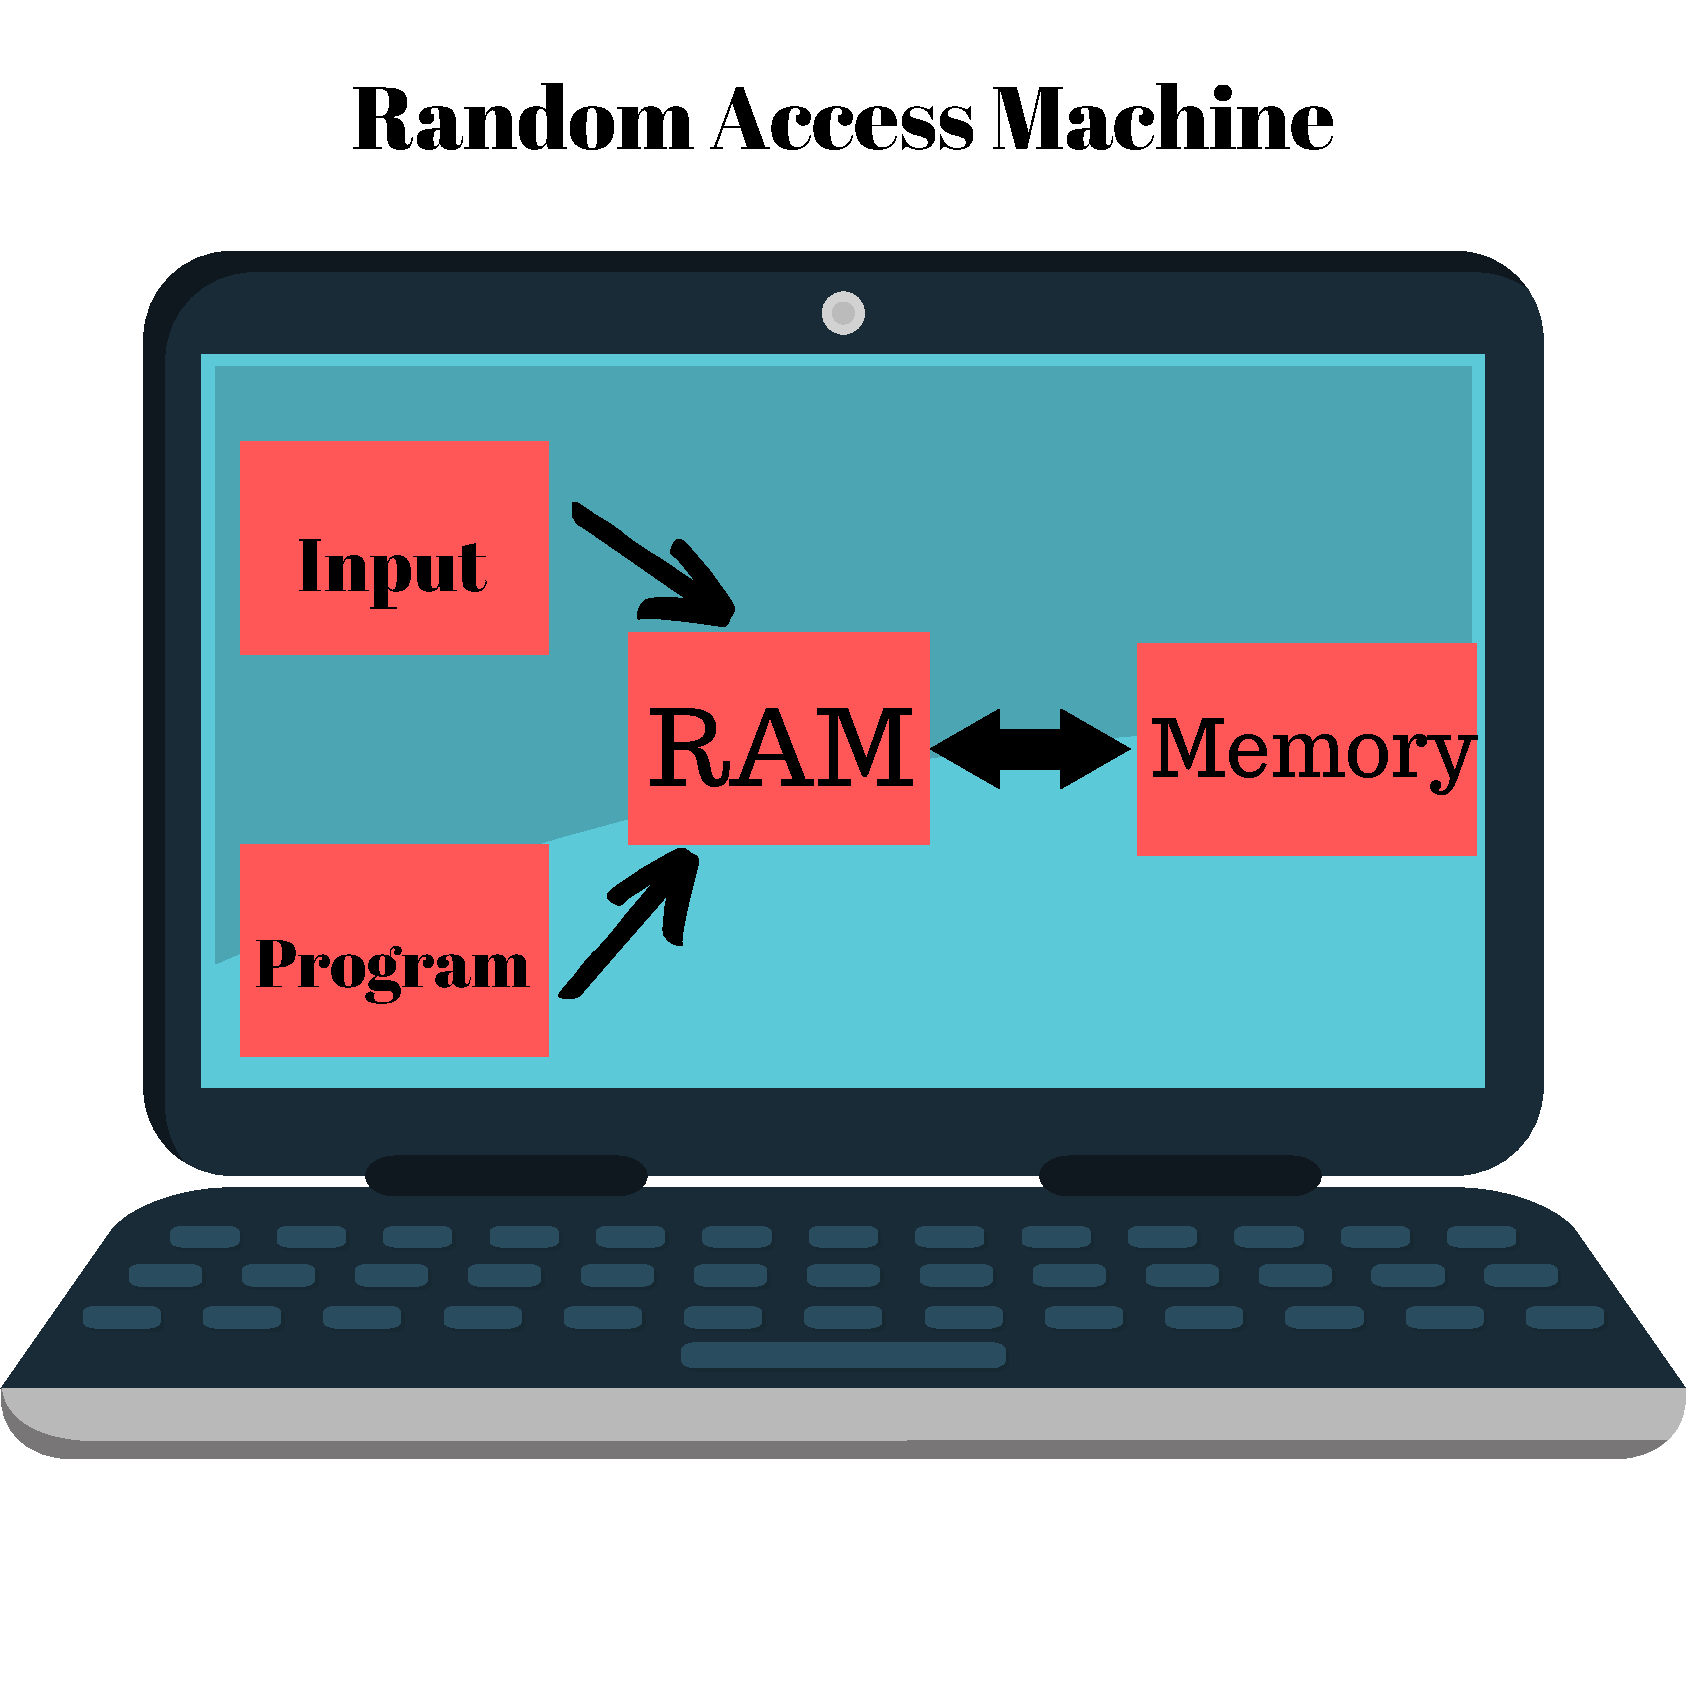
\includegraphics[width=90mm]{Pictures/RAM_1.pdf}
\end{figure}
\vspace{1em} 
\begin{definition}
Basic operations such as addition, multiplication, load, store,
copy, control, initialization are assumed to take a constant
amount of time each (if numbers are big, this may not be true,
but we assume that this is the case unless stated otherwise).
\end{definition}
\begin{remark}
Not to be confused with \textbf{Random Access Memory} 
\end{remark}
\textbf{Solution:}
\begin{itemize}
    \item The RAM (Random Access Machine) model is used for analyzing algorithms where we assume  that instructions are executed one after the other. It is used to model how real world programs would run.
    \item Machine independent and theoretical.
    \item Simple operations such as $(+,\times, -, =)$ take $O(1)$ time.
    \item Loops and subroutines are not considered simple operations. Instead, they are the composition of many single-step operations
\end{itemize}
%------------------------------------------------
\subsection{Merge Sort}
\begin{example}
Show the operation of Merge sort on the array  $A= <7,4,2,8,3,1,5,6,9>$
\end{example}
\begin{definition}
\textbf{Merge Sort} A divide and conquer algorithm. Takes an input array and divides it into two halves, calls itself for the two halves, and merges the two sorted halves. 
\begin{itemize}
    \item \textbf{merge()} function merges two halves. 
    \item \textbf{MergeSort()} function recursively calls itself to divide the array until its size becomes one. 
\end{itemize}
\end{definition}
\begin{lstlisting}[caption={Merge-Sort(A,p,r)}, escapeinside={(*}{*)}]
if p < r 
    q = (*$\floor[\Big]{(p + r)/2}$*)
    Merge-Sort(A,p,q)
    Merge-Sort(A,q+1,r)
    Merge(A,p,q,r)
\end{lstlisting}
\vspace{1em} 
\textbf{Solution:} 
\begin{comment}
$$\text{Sorted}$$
    $$[1][2][3][4][5][6][7][8][9]$$
    $$[2][4][7][8] \qquad [1][3][5][6] \qquad[9]$$
    $$[4][7] \qquad [2][8] \qquad [1][3] \qquad [5][6]\qquad[9]$$
    $$[7]\qquad [4]\qquad [2]\qquad [8]\qquad [3]\qquad [1]\qquad [5]\qquad [6]\qquad [9]$$
    $$[7]\qquad [4]\qquad [2]\qquad [8]\qquad [3]\qquad [1]\qquad [5]\qquad [6][9]$$
    $$[7][4]\qquad[2][8]\qquad[3][1]\qquad[5][6][9]$$
    $$[7][4][2][8]\qquad[3][1][5][6][9]$$
    $$[7][4][2][8][3][1][5][6][9]$$
$$\text{Unsorted}$$
\end{comment}
\begin{figure}[H]
    \centering
    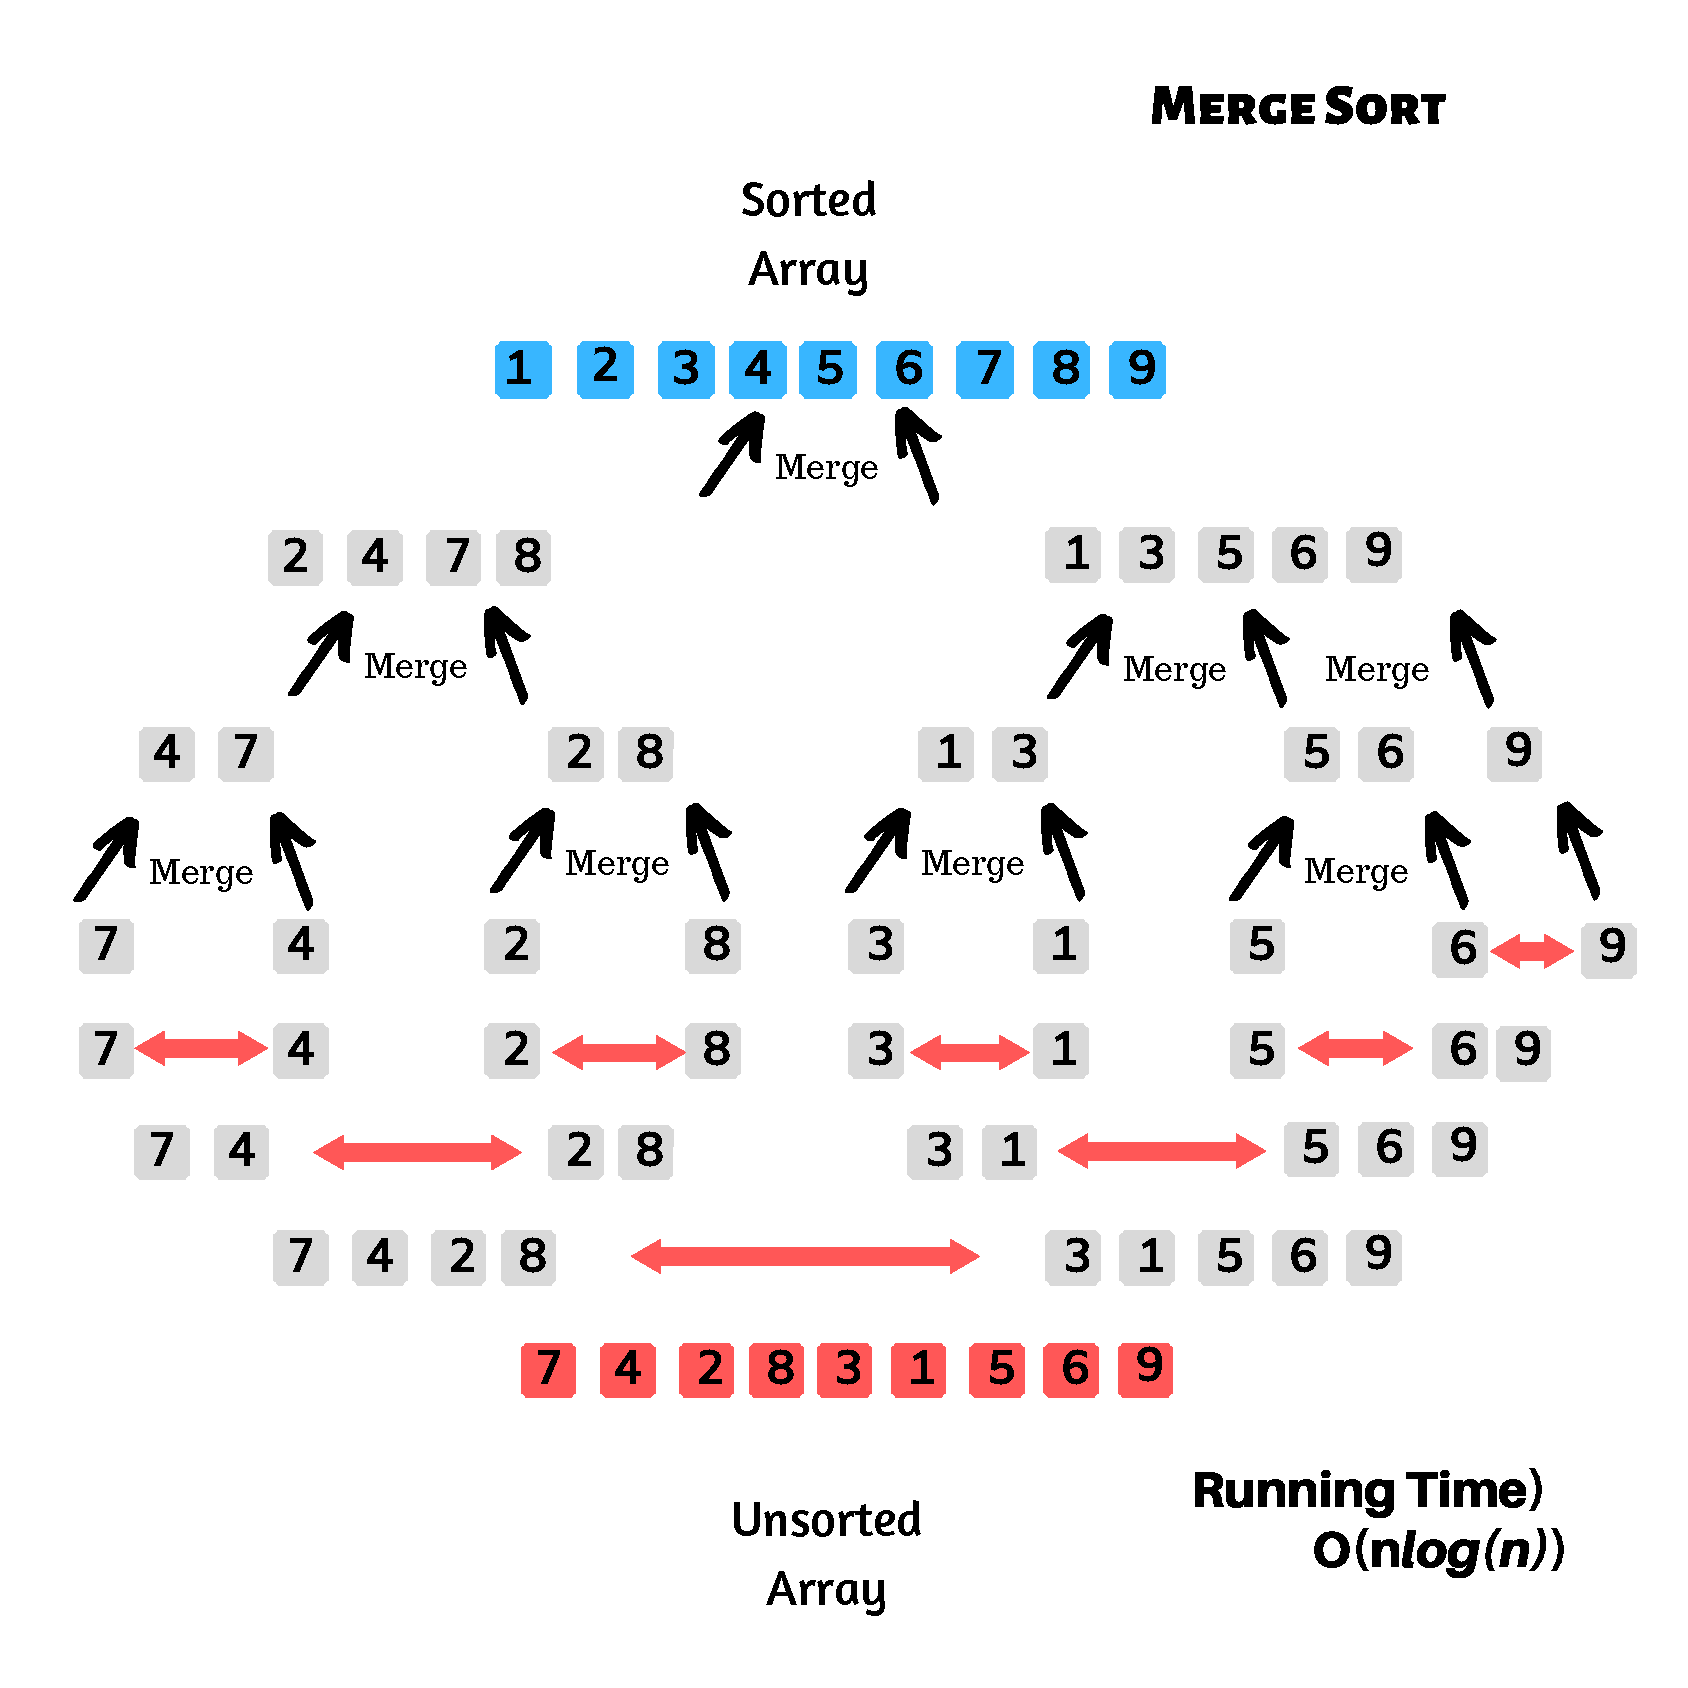
\includegraphics[width=150mm]{Pictures/1.pdf}
    %\caption{Caption}
    %\label{fig:my_label}
\end{figure}
\begin{example}
 \textit{Merge Sort} is always faster than \textit{Insertion Sort}.  True or false?. \\ Justify your answer
\end{example}
\begin{definition}
\textbf{Time Complexity} is the computational complexity that describes the amount of time it takes to run an algorithm. Time complexity is commonly estimated by counting the number of elementary operations performed by the algorithm, supposing that each elementary operation takes a fixed amount of time to perform.
\end{definition}
\begin{center}
Big-O Time Complexity Graph
\end{center}
\begin{tikzpicture}
\begin{axis}[
    axis lines = left,
    xlabel = Elements,
    ylabel = {Operations},
    title = \textbf{Best Case} ,
]

\addplot [
    domain=1:20, 
    samples=200, 
    color=red,
]
{x*ln(x)};
\addlegendentry{Merge Sort : $O(n\log(n))$}
\addplot [
    domain=1:20, 
    samples=200, 
    color=blue,
    ]
    {x};
\addlegendentry{Insertion Sort : $O(n)$}

\end{axis}
\end{tikzpicture}
\\
\begin{tikzpicture}
\begin{axis}[
    axis lines = left,
    xlabel = Elements,
    ylabel = {Operations},
    title = \textbf{Average \& Worst} ,
]

\addplot [
    domain=1:20, 
    samples=200, 
    color=red,
]
{x*ln(x)};
\addlegendentry{Merge Sort : $O(n\log(n))$}
\addplot [
    domain=1:20, 
    samples=200, 
    color=blue,
    ]
    {x^2};
\addlegendentry{Insertion Sort : $O(n^2)$}
 
\end{axis}
\end{tikzpicture}
\begin{remark}
When asked for running time of an algorithm this refers to $O(\cdot)$. Runtime time means worst case running time. 
\end{remark}
\vspace{1em}
\textbf{Solution: } 
False: Merge sort is not always faster than insertion sort. In the \textbf{Best Case} Merge Sort's running time is $O(n\log(n)$ and Insertion Sort is linear $O(n)$. For \textbf{Average Case} and \textbf{Worst Case} Merge Sort is faster. 
\subsection{Insertion Sort vs Merge Sort}
\begin{example}
Suppose the input sequence is already sorted.  For this specific input, what is the running time of Insertion-sort and Merge-sort?. Consider \textit{listing 1.1 and 1.2}
\end{example}
\begin{figure}[H]
    \centering
    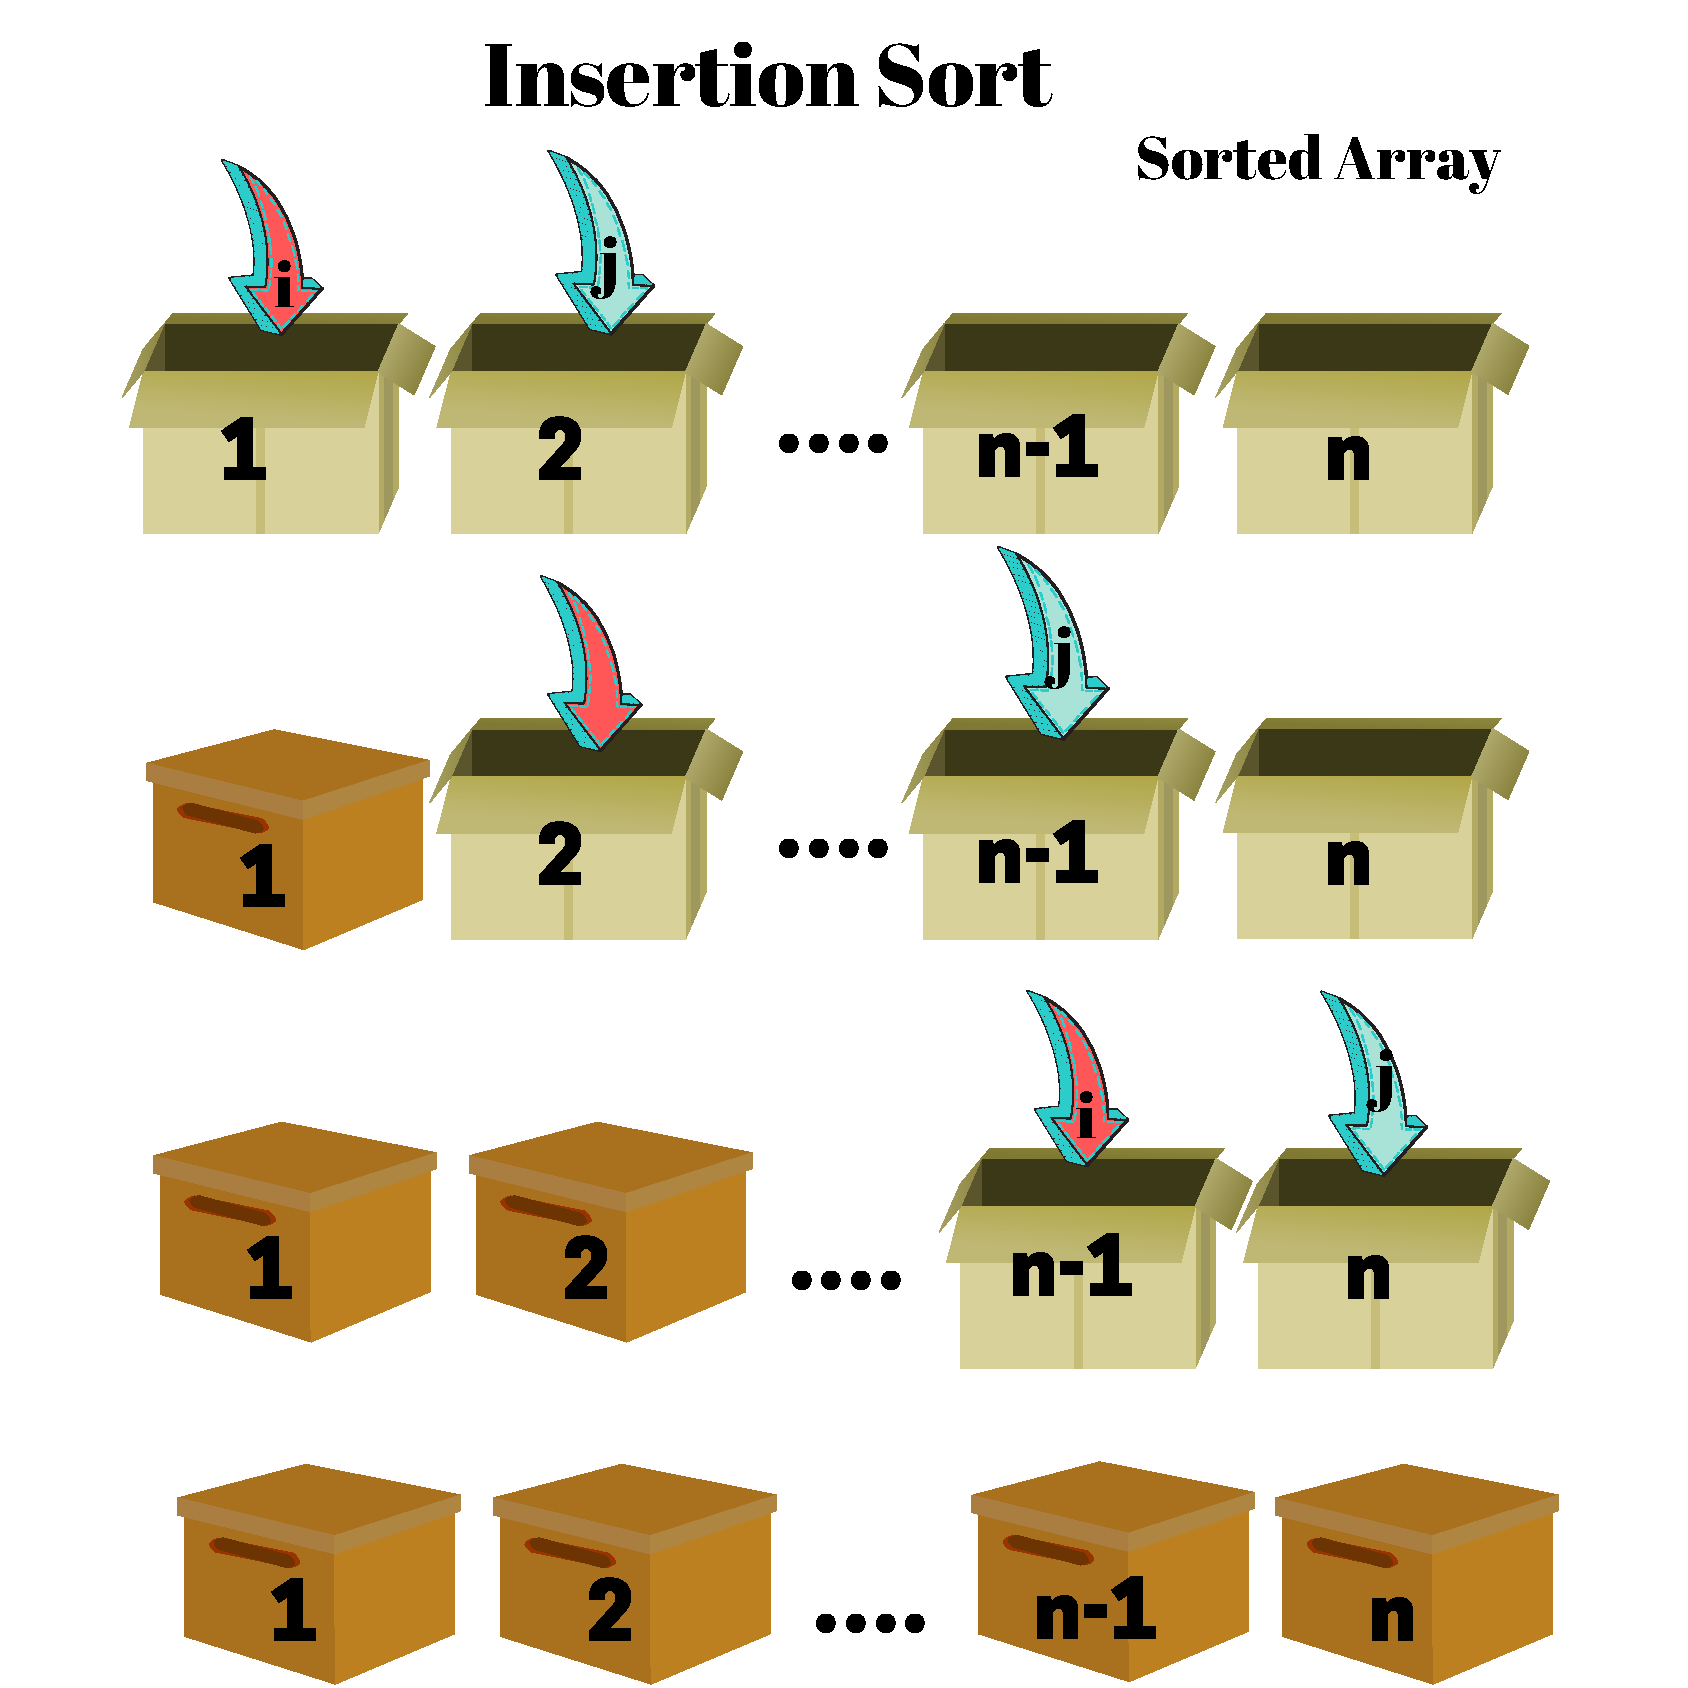
\includegraphics[width=100mm]{Pictures/SortedInsertion.pdf}
\end{figure}
\textbf{Solution:} For insertion sort the running time is $\Theta(n)$, for merge sort it is $\Theta(n\log(n))$.
\begin{itemize}
    \item \textit{Insertion Sort} must iterate through the entire array.
    \item The while loop (\textbf{Lines 6-8}) of Insertion Sort (\textit{Listing 1.1} ) does not execute.
\end{itemize}
\subsection{Running Time}
\begin{example}
Suppose there are $2^n$ inputs to a certain problem. The running time of an algorithm A is exactly $2^n$ for exactly one of the inputs, and 1 for any other input. Then the running time is O(1) since $2^n \cdot \frac{1}{2^n} + 1\cdot(1 - \frac{1}{2^n}) \leq 2$. Is this statement correct?
\end{example}
\textbf{Solution:} 
False: The statement is in correct. O notation refers to worst case running time, this means the running time for the algorithm is $O(2^n)$ .
\section{Intermediate}\index{Intermediate}
\subsection{Selection-Sort}
\begin{example}
 The following is a pseudo-code of Selection-Sort.  Describe Selection-Sort in plain English.
\end{example}
\textbf{Solution:} 
 \begin{lstlisting}[caption={Selection-Sort(A)}, escapeinside={(*}{*)}]
 n = A.length 
 for (*$j = 1$*) to (*$n - 1$*)
    smallest = j 
    for (*$i = j + 1$*) to n 
        if (*$A[i] < A[smallest]$*)
            smallest = i 
    exchange A[j] with A[smallest]
\end{lstlisting} 
    Selection sort finds the smallest element in the array and swaps it with the first element, then the second smallest with the second element, third smallest swaps with third element and so on. 
    \vspace{1em}
        For selection sort the array of size n is iterated from the first index in the array to the one before the last index. It is assumed that the first index is the smallest, then the next elements are compared to the first element and if it is smaller then that index becomes the smallest, and this continues until every element after is tested. Then the element at index j is swapped with the smallest element.  
\begin{example}
State the loop invariant and prove that the algorithm is correct. What is the running time?
\end{example}
\begin{enumerate}
    \item We want to show that the loop invariant is true prior to the first iteration of the loop, that each iteration maintains the loop invariant, and that the loop invariant gives us a useful property at loop termination.\\ \\
        Loop Invariant: $A[\text{smallest}] \leq A[1..j-1]$
        \begin{itemize}
            \item \textbf{Initialization} Prior to the first iteration A[1] is sorted. When j = 1 there is only one element and is therefore sorted. In the second for loop, i = j + 1, $A[1..j-1]$, it is only $A[i]$, one element only. 
            \item \textbf{Maintenance} It remains true as j increases and i is the element after j. The outer loop from j = 1 to n -1 and i = j + 1 to n, the inner loop finds smallest element from j + 1 and the outer loop exchanges the jth element with the smallest element. The sub-array A[1..j] is sorted. 
            \item \textbf{Termination} The sub-array A[1..n] is sorted, the outer loop iterates from j = 1 to n -1 
        \end{itemize}
        \item The worst case running time is $O(n^2)$ and best case is $\Omega(n^2)$. The average case is $\Theta(n^2)$ 
\end{enumerate}
\subsection{Merge}
\begin{example}
Consider the pseudo-code of Merge(A, p, q, r) in the textbook.  Given that A[p...q] and A[q+ 1...r] are both sorted, the function call merges the two sorted sub arraysinto a sorted subarray A[p...r].  Prove the correctness of Merge.  For simplicity,  you can assume that $L[1...n_1]$ = $A[p...q]$ and $R[1...n_2]$ = $A[q+1...r]$., and $L[n_1+1]$ = $R[n_2+1] = \infty$. (So you only need to consider from lines 10).  You can assume that all elements stored in the array have distinct values. 
\end{example}
\textbf{Solution: } 
MERGE(A,p,q,r)
    \begin{lstlisting}
    n_1 = q - p + 1
    n_2 = r - q
    let L[1..n_1 + 1] and R[1..n_2 + 1] be new arrays 
    for i = 1 to n_1 
        L[i] = A[p + i - 1]
    for j = 1 to n_2 
        R[j] = A[q + j]
    L[n_1 + 1] = \infinity 
    R[n_2 + 1] = \infinity
    i = 1 
    j = 1 
    for k = p to r 
        if L[i] <= R[j]
            A[k] = L[i]
            i = i + 1
        else A[k] = R[j]
            j = j + 1
    \end{lstlisting} 
    \vspace{1em}
    Loop Invariant: $k \in [p,r]$ elements in index k are sorted, this elements come from Left and Right subarrays, also $i <= n_1 + 1, j \leq n_2 + 1$ where $i \in [p,q], j \in [q+1,r]$ this means there are no more elements to be copied to A[p..r].
    \vspace{1em}
\begin{enumerate}
    \item Initialization : Our merged array $A[p..r]$ before line 10 contains no elements from our sorted sub arrays $A[i] , A[j]$ recall that elements were stored in new sub arrays $L[1..n_1]$ or $R[1..n_2]$ and therefore $A[k]$ is "empty", therefore sorted. 
    \item Maintenance :  The for loop iterates from $k \in p to r$, and elements are added to A[k], we must show this loop invariant is in sorted order. Check by Iterating through each element in L[i] and R[j] and finding the smallest element after the first iteration A[p] holds one single element, this element is sorted since it belongs to the smallest element of subarray L[1..$n_1$] or subarray R[1..$n_2$]. 
    \item Termination : The loop iterate through (r - p + 1) element's and compares each element in the subarrays $L[1..n_1$ and $R[1..n_2$ to find the smallest, then it is stored in the array A[p..r], at the end of
\end{enumerate}
%------------------------------------------------

\section{Advanced}\index{Advanced}
\subsection{Searching Problem}
\begin{example}
Consider the searching problem The input is an array A[1..n] of n numbers and a value v. You're asked to find an index i such that A[i] = v. If there's no such index, return NIL. The following is a pseudocode of linear search, which scans through the sequence, looking for v. Using a loop invariant, prove that your algorithm is correct. Make sure that your loop invariant fulfills the there necessary properties. What is the asymptotic worst case running time? 
\end{example}
\textbf{Solution: } 
\begin{lstlisting}
    For i = 1 to n
        If A[i] == v then return i 
    return NIL
\end{lstlisting}
\begin{enumerate}
        \item Loop Invariant: 
        At the start of each \textit{ith} iteration of the for loop $j \in [1, i-1]$ and A[j] is not v.
        \begin{enumerate}
        \item Initialization : Before the loop iteration the \textbf{variable answer} contains NIL,that is since $j = 0 \rightarrow A[0]$ does not exist. A[0] is therefore not v.
        \item Maintenance : Assume the loop invariant holds then $A[j]$is not v. If $A[j+1]$ is v then the termination would have followed. Since termination has not followed (loop is still running) this implies that $A[j+1]$ is not v. 
        \item Termination : When the for loop terminates the variable answer contains v or NIL.It returns NIL if at index j + 1 the element is v, or returns NIL if at index j + 2 which is larger than the size of array and therefore A[j+2] is not v. 
        \end{enumerate}
        \item The asymptotic worst case is $O(n)$, that is the element is at the index n, it must examine every element. 
\end{enumerate}
%\section{Supplemental Problems} 
\section{Exam Problems} 
\subsection{Insertion Sort}
\begin{example}
The following is a pseudocode of Insertion-Sort for instance A[1..8] = $\langle 7,4,2,9,4,3,1,6\rangle$ what is $A[1..8]$ just before the for loop starts for j = 5?
\vspace{1em}
\\
\textbf{INSERTION-SORT(A)}
\begin{lstlisting}
for j = 2 to A.length
    key = A[j]
    //insert A[j] into the sorted
        sequence A[1..j-1]
    i = j - 1
    while i > 0 and A[i] > key
        A[i+1] = A[i]
        i = i - 1
    A[i+1] = key
\end{lstlisting}
\end{example}
\textbf{Solution:}
\vspace{1em}
\begin{tabular}{c|c}
    j & After \\
    j = 2 & $\langle 4,7,2,9,4,3,1,6 \rangle$ \\
    j = 3 & $\langle 2,4,7,9,4,3,1,6 \rangle$ \\
    j = 4 & $\langle 2,4,7,9,4,3,1,6\rangle$ \\
    j = 5 & $\langle 2,4,4,7,9,3,1,6 \rangle$ \\
\end{tabular}
\\
Before j = 5 the array $A[1..8]$ is $\langle 2,4,7,9,4,3,1,6\rangle$
\begin{example}
Give an instance of size n for which the insertion-sort terminates in $\Omega(n^2)$
\end{example}
\textbf{Solution:} The input should be n numbers in decreasing order. The while loop executes.  \\
Example: $\langle 6,5,4,3,2,1 \rangle$
\begin{example}
Give an instance of size n for which the Insertion-sort terminates in $O(n)$ time.
\end{example}
\textbf{Solution:} The input should be n number in increasing order. The while loop does execute.\\
Example: $\langle 1,2,3,4,5,6 \rangle$
\begin{example}
The following is a pseudocode of Insertion-sort. Prove its correctness via loop invariant. In other words, state the loop invariant and prove it using \textit{Initialization, Maintenance, and Termination}\\
\textbf{INSERTION-SORT(A)}
\begin{lstlisting}
for j = 2 to A.length 
    key = A[j]
    //Insert A[j] into the sorted 
        sequence A[1..j-1]
    i = j - 1
    while i > 0 and A[i] > key
        A[i + 1] = A[i]
        i = i - 1
    A[i + 1] = key 
\end{lstlisting}
\end{example}
\textbf{Solution:}
Loop Invariant: At the start of each of the \textbf{for} loop of lines 1 -8, the subarray A[1..j-1] consists of the elements originally in A[1..j-1], but in sorted order. 
\begin{enumerate}
    \item \textbf{Initialization} Just at the start of the first iteration (j=2), A[1] is ordered and the number was originally in A[1].
    \item \textbf{Maintenance} Say the invariant is true for iteration $j \geq 2$. At the end of the iteration. The algorithm has $A[1..i]$, A[j], and A[i+1..j-1] in this order in the prefix of A. We know that $A[1..i]$ and $A[i + 1..j-1]$ are sorted by the invariant. Further, $A[i] \leq A[j] \leq A[i + 1]$ by Algo's definition, meaning A[1..j] is sorted at the end of iteration. Clearly, all elements in $A[1..j]$ originate form the same subarray. Thus, the loop invariant holds before the next iteration j + 1/ 
    \item \textbf{Termination} The for loop ends when j = n + 1, and the loop invariant implies that the array is sorted as desired. 
\end{enumerate}
\subsection{RAM - Random Machine Model} 
\begin{example}
Briefly explain the Random Access Model (RAM)
\end{example}
\textbf{Solution:}
The RAM model is used for analyzing algorithms where we assume  that instructions are executed one after the other. This model is theoretical.It is used to model how real world programs would run.\\
Basic operations such as addition, multiplication, load, store,
copy, control, initialization are assumed to take a constant
amount of time each (if numbers are big, this may not be true,
but we assume that this is the case unless stated otherwise).
\subsection{Merge Sort} 
\begin{example}
Let T(n) denote the running time of Merge-sort on input size n. In the following you can omit floor or ceeling. 
MERGE-SORT(A,p,r)
\begin{lstlisting}
if p < r 
    q = floor((p+r)/2)
    MERGE-SORT(A,p,q)
    MERGE-SORT(A,q+1,r)
    MERGE(A,p,q,r)
\end{lstlisting}
\end{example}
\begin{remark}
\textbf{Running time of Merge Sort} 
\[
f(a,b) = 
     \begin{cases}
       O(1) &\quad\text{if } n = 1\\
       2T(n/2) + \Theta(n) &\quad\text{if }  n \geq 2 \\
     \end{cases}
\]
\end{remark}
\begin{enumerate}
    \item What is the running time of Line 3 (of Merge-Sort)? \\
    \textbf{Solution:} A call to merge sort is $T(n/2)$
    \item What is the running time of Line 4 (of Merge-Sort)?\\
     \textbf{Solution:} A call to merge sort is $T(n/2)$
    \item What is the running time of LIne 5 (of Merge-Sort)?\\
     \textbf{Solution:} A call to merge is $\Theta(n)$
\end{enumerate}
\section{Solutions To Exercises}
%----------------------------------------------------------------------------------------
%	CHAPTER 2
%----------------------------------------------------------------------------------------

\chapter{ Growth of Functions}

\section{Basic}\index{Basic}
\subsection{Ranking Functions}
\vspace{1em}
\begin{example}
Rank  the  following  functions  by  order  of  growth;  that  is,  find  an  ordering $g_1, g_2, \cdot \cdot \cdot, g_k$ (here k is the number of functions given) such that $g_1 = \mathcal{O}(g_2), g_2$ = $\mathcal{O}(g_3), \cdot \cdot \cdot, g_{k - 1}$ = $\mathcal{O}(g_{k}) $ (For  example,  if  you  are  given  functions, $n^2, n,2n,$  your solution should be either $n,2n, n^2$ or $2n, n, n^2$.) 
\begin{center}
    \begin{tabular}{c|c|c|c|c|c}
        $n^2 + 2^n$  &  $n\log(n)$ & $n^2(\log(n))^2$ & $n(\log(n))^2$ & $n^2$ & $log^{100}(n)$\\
        $\log(\log(n))$ & $n^3$ & 1 & $\log(n)$ & $\frac{\log(n)}{\log\log(n)}$ & $\frac{n^2}{log(n)}$\\
        $n^{10}3^{n}$ & $4^n$ & & & &
    \end{tabular}
\end{center}
\textbf{Solution:} \\
\begin{enumerate}
    \item \textbf{Asymptotic upper bound}. $\mathcal{O} - notation$
    $$\mathcal{O}(g(n)) \text{ = } \{f(n) : \text{there exist positive constants c and } n_o \text{ such that } 
    0 \leq f(n) \leq c(g(n) \text{for all} n \geq n_o\}$$
    \item We consider the following. (Algorithm Design Manual, Page 40) $$1 \text{ << } \log(n) \text{ << } n \text{ << } n\log(n) \text{ << } n^2 \text{ << } n^3 \text{ << } 2^n \text{ << } n!$$ 
    \item Find $g_1$ the smallest function. Since $1$ is a constant it is the smallest function. Therefore $$g_1 \text{ = } 1$$
    \item Find $g_2$. We know that $\log(n)$ is smaller than n, so $\log(\log(n))$ is smaller than $\log(n)$ Therefore 
    $$g_2 \text{ = } \log(\log(n))$$
    \item Find $g_3, g_4, g_5$
    \begin{itemize}
        \item Candidates are $\log(n)$, $\log^{100}(n)$ and $ \frac{\log(n)}{\log(\log(n))}$
        \item $\log(n) \text{ < } (\log(n))^{100}$. 
        \item We find $\frac{\log(n)}{1} \text{ > } \frac{\log(n)}{\log(\log(n))}$. Recall if that the larger the denominator the smaller the value.
        \item Therefore we know that $\frac{\log(n)}{\log(\log(n))} \text{ < } \log(n) \text{ < }  (\log(n))^{100} $
        $$g_3 \text{ = } \frac{\log(n)}{\log(\log(n))}, g_{4} \text{ = } \log(n) , g_5 \text{ = } (\log(n))^{100}$$
    \end{itemize}
    \item Find $g_6, g_7$
        \begin{itemize}
            \item Find all functions that have \textit{n}. There are no values with n. 
            \item Possible candidates $n\log(n), n(\log(n))^2$. $$n\log(n) \text{ < }  n(\log(n))^2$$
            $$g_6 \text{ = }  n\log(n) , g_7 \text{ = }  n(\log(n))^2$$
        \end{itemize}
    \item Find $g_8, g_9, g_10$
    \begin{itemize}
        \item Find functions that contain $n^2$. Potentially $n^2, n^2(\log(n))^2, \frac{n^2}{\log(n)}$
        \item Since $\frac{n^2}{\log(n)} \text{ < }  n^2$
        \item And $n^2 \text{ < }  n^2(\log(n))^2 $
        \item Therefore $g_8$ = $\frac{n^2}{\log(n)}, g_9 \text{ = }  n^2, g_{10} \text{ = }  n^2(\log(n))^2$
    \end{itemize}
    \item Find $g_{11}, g_{12}, g_{13}, g_{14}$
    \begin{itemize}
        \item Find functions with $n^3$. Only $n^3$ is left. $$g_{11} \text{ = }  n^3$$
        \item Find functions with $2^n$. Functions $n^2 + 2^n, 2^n$. Therefore 
        $$g_{12} \text{ = } 2^n, g_{13} \text{ = } n^2 + 2^n$$
        \item Finally $g_{14} \text{ = } n^{10}3^n$
    \end{itemize}
    \color{blue}
    Solution: $$1, \log(\log(n)), \frac{\log(n)}{\log(\log(n))}, \log(n), (\log(n))^{100}, n\log(n), n(\log(n))^2, \frac{n^2}{\log(n)}, n^2, n^2(\log(n))^2, n^3, 2^n, n^2 + 2^n$$ 
    \large
    \color{black} 
\end{enumerate}
\end{example}
\subsection{Asymptotically no smaller}
\begin{example}
 What is $\lim_{n \to \infty} \frac{n^{10}\cdot 3^n}{4^n}$?  Which one is asymptotically no smaller between the two functions?
\end{example}
\textbf{Solution:}
\begin{enumerate}
    \item Consider the following \\
    $$\lim_{n \to \infty} \frac{f(n)}{g(n)} \text{ = } 0, \text{implies} f(n) \text{ = } O(g(n))$$
    \item $$\lim_{n \to \infty} \frac{n^{10}3^n}{4^n} \text{ = } 0 $$
    \item Since $4^n\text{ > } n^{10}3^n$
    \item $g \text{ = } \Omega(n^{10}3^n)$
    \item $f \text{ = } O(4^n)$
\end{enumerate}
The limit is $0$, and the function that is asymptotically no smaller between the two functions is $f \text{ = } O(4^n)$ since $4^n$ is the upper bound and $n^{10}3^n$ is the lower bound. 
\subsection{Using asymptotic definitions}
\begin{example}
Formally prove that $n^2+ 100 \text{ = }\mathcal{O}(n^2)$ using the definition of $\mathcal{O}(\cdot)$
\end{example}
\textbf{Solution:}
\begin{enumerate}
    \item Consider the following. \\
    \begin{definition}
     $\mathcal{O}(g(n))$ = $\{f(n)$ : there exist positive constants c and  $n_o$ such that\\ $
    0 \leq f(n) \leq c(g(n) \text{for all} n \geq n_o\}$
    \end{definition}
    \item We want to show that $0 \leq n^2 + 100 \leq c\cdot n^2$
    $$n^2 + 100 \leq c\cdot n^2$$
    $$100 \leq n^2(c - 1) $$
    $$0 \text{ < } \frac{100}{c - 1} \leq n^2$$
    \item A c was chosen by inspection, then you may use c to solve the inequality and solve for n. 
    \item If $c \geq 101 $ then $1 \leq n^2$ this holds true for $n \geq 1$, therefore we have $n^2 + 100 \leq 101n^2$
\end{enumerate} 
    \color{blue}Solution:  Since  c , and $n_0$ exist where  $n \geq n_0$ that is $n^2 + 100 \leq 101n^2 $\color{black}
\begin{example}
Formally prove that $n^2= \Omega(n^2+ 100)$ Using the definition of $\Omega(\cdot)$.
\end{example}
\textbf{Solution: } 
\begin{enumerate}
    \item Consider the following. \\
    \begin{definition}
    $\Omega(g(n) \text{ = } \{f(n) : $ there exist positive constants c and $n_0$ such that $0 \leq cg(n) \leq f(n)$ for all $n \geq n_0$
    \end{definition}
    \item We want to show that $0 \leq c(n^2 + 100) \leq n^2$ by finding a c and $n_0$ such that $n \geq n_0$
    $$0 \leq c(n^2 + 100) \leq n^2$$
    $$cn^2 + 100c \leq n^2$$
    \item Choose a c by inspection.If c is 1, it does not hold. Less than one, we want $100c$ to head to zero. Therefore, choose $ c= \frac{1}{101}$ meaning $\frac{n^2}{100} + \frac{100}{101} \leq n^2 $
    \item $c \text{ = }  \frac{1}{101}$ means $$\frac{1}{101}(n^2 + 100) \leq n^2$$
     $$n^2 + 100 \leq 101n^2$$
     $$100 \leq  100n^2$$
     $$1 \leq  n^2 \rightarrow \pm 1 \leq n$$
     \item for $c \text{ = }  \frac{1}{101}, n \geq 1 $
\end{enumerate}
\color{blue} Solution: There exists a c and a $n$, this means the definition holds.In turn  $\frac{1}{101}(n^2 + 100) \leq n^2$
\color{black}
\begin{example}
 Formally prove that $n^2 \text{ = }\Omega(n\log_2n + 100)$ using the definition of $\Omega(\cdot)$
\end{example}
\begin{enumerate}
    \item Consider the following. \\
    \begin{definition}
    $\Omega(g(n) \text{ = } \{f(n) : $ there exist positive constants c and $n_0$ such that $0 \leq cg(n) \leq f(n)$ for all $n \geq n_0$
    \end{definition}
    \item We want to show that $0 \leq c(n\log_2(n) + 100) \leq n^2$
    $$c(n\log_2(n) + 100) \leq n^2$$
    \item Algebra: Distribute c, then Raise every-ting to the power of 2, to cancel the $log_2$. Recall $2^{a + b} \text{ = } 2^a2^b$. Recall properties of log. $a\log_2{b} \rightarrow \log_2{b^a}$
    $$2^{\log_2(n^{cn})}2^{100c}) \leq 2^{n^2}$$
    $$n^{cn}2^{100c} \leq 2^{n^2}$$
    \item Choose a c by inspection. 
    \item If $c \text{ = } 1$ then 
    $$n^{n} \leq 2^{n^2 - 100}$$
    $$n\log_2{n} \leq n^2 - 100$$
    $$0 \leq n^2 - n\log_2(n) - 100$$
   \item It holds for some n, unable to find. Come back later. 
\end{enumerate}
\begin{example}
 Formally prove that $n + 10 = \Theta(50n + 1)$ using the definition of $\Theta(\cdot)$
\end{example}
\textbf{Solution: } 
\begin{enumerate}
    \item Consider the following. 
    \begin{definition}
    $\Theta(g(n)) = \{ f(n) : $ there exist positive constants $c_1, c_2$ and $n_0$ such that\\ $c_1g(n) \leq f(n) \leq c_2g(n)$ for all $n \geq n_0$ \\\\
    $f(n) = \Theta(g(n)) \text{ iff } f(n) = \Omega(g(n)) \text{ and } f(n) = \mathcal{O} g(n)$
    \end{definition}
    \item We want to show that $c_1(50n + 1) \leq n + 10 \leq c_2(50n + 1)$
    \item Proving $\Omega$ and $\mathcal{O}$ makes it easier.
    \item First prove the upper bound $\mathcal{O}$. 
    $$n + 10 \leq c_2(50n + 1)$$
    %To find a $c$ do the following $$\lim_{n \to \infty} \frac{n + 10}{50n + 1} \leq c_2$$
    If $c_2 = 1$ and $n \geq 1 \rightarrow n + 9 \leq 50n$ holds. 
    
    \item Second prove the lower bound $\Omega$. 
    $$c_1(50n + 1) \leq n + 10$$
    \item  If $c_1 = \frac{1}{50}$ then for $n + \frac{1}{50} \leq n + 10 $
\end{enumerate}
\color{blue} Solution: Since we have found a $c_1, c_2, n$ the definition is met. Therefore $$\frac{1}{50}(50n + 10) \leq n + 10 \leq 50n + 1 $$ \color{black}
\section{Intermediate}
\subsection{Using big-O notation}
\begin{example}
 Prove that $f = O(g)$ implies $g = \Omega(f)$
\end{example}
\begin{enumerate}
    \item $f(n) = O(g(n)), g(n) = \Omega(f(n)$\\ Meaning that if g(n) is the upper bound then this implies $f(n)$ and $f(n)$ is the lower bound of $g(n)$ 
    \item \color{blue} Solution : $f(n) \leq c_1 g(n) \text{ Definition of O} \rightarrow \frac{1}{c_1} f(n) \leq g(n) \rightarrow c_2 f(n) \leq g(n) \text{ Definition of } \Omega$\\ (note $c_2 = \frac{1}{c_1})$\color{black} 
\end{enumerate}
\begin{example}
Prove that $f = \Omega(g)$ and $g = \Omega(h)$ implies $f = \Omega(h)$ 
\end{example}
\begin{enumerate}
    \item $g = \Omega(h)$ means $0 \leq ch(n) \leq g(n)$ for $n_1 > n_0$
    \item $f = \Omega(g)$ means $0 \leq cg(n) \leq f(n)$ for $n_2 > n_0$
    \item $f = \Omega(h)$ means $0 \leq ch(n) \leq f(n)$ for $n_2 > n_1$
\end{enumerate}
%\section{Miscellaneous Problems}
\section{Exam Problems} 
\subsection{True or False}
For each of the following claims, decide if it is true or false. No explanation is needed.\\
\textbf{To solve consider the following}
\begin{enumerate}
    \item \textbf{Dominance Pecking Order} \textit{Page 56, Algo Design Manual}
    $$1 < \alpha(n) < \log(\log(n)) < \frac{\log(n)}{\log(\log(n))} <  \log(n) <  \log^2(n) $$
    $$< \sqrt{n} < n < n\log(n) < n^{1 + \epsilon}  < n^2 < n^3 < c^n < n!$$
    \item \textbf{Asymptotic Upper Bound} 
    \begin{definition}
    $f(n) = O(g(n))$means $c\cdot g(n)$ is an \textit{upper bound} on f(n). Thus there exists some
    constant c such that f(n) is always $\leq c\cdot(n),$ for large enough n (i.e.., $n\geq n_o$ for some constant $n_0$).
    \end{definition}
    \item \textbf{Asymptotic Lower Bound}
    \begin{definition}
        $\Omega(g(n)) = \{f(n): $ there exist positive constant c and $n_0$ such that \\
        $0 \leq cg(n) \leq f(n)$ for all $n \geq n_0$
    \end{definition}
    \item \textbf{Asymptotically tight bound } 
    \begin{definition}
        $\Theta(g(n)) = \{ f(n) : $ there exist positive constants $c_1, c_2$ and $n_0$ such that\\ $c_1g(n) \leq f(n) \leq c_2g(n)$ for all $n \geq n_0$
    \end{definition}
\end{enumerate}
\begin{example}
$n\log(n) = O(n^2)$
\end{example}
\textbf{Solution:} True, since $n\log(n) < c\cdot n^2$
\begin{example}
$\log(\log(n)) = O(\log(n))$
\end{example}
\textbf{Solution:} True, since $\log(\log(n)) < c\cdot \log(n)$
\begin{example}
$\log^{50}n = O(n^{0.1})$
\end{example}
\textbf{Solution:} True, since $\log^{50}n \leq c(n^{0.1}))$
\begin{example}
$4^n = O(2^n)$
\end{example}
\textbf{Solution:} False, since $4^n \not\leq c\cdot(2^n)$
\begin{example}
$100^{100} = \Theta(1)$
\end{example}
\textbf{Solution:} True, since $100^{100} \leq c \cdot 1$
\begin{example}
If $f = O(g)$, then $g = \Omega(f)$
\end{example}
\textbf{Solution:} True. If $f \leq c g(n)$ then $g(n)$ is the upper bound, this implies that $f(n)$ 
is the lower bound, therefore $g \geq c f(n)$
\begin{example}
If $n^3 = \Omega(n^2)$
\end{example}
\textbf{Solution:} True, since $n^3 \geq c \cdot(n^2)$
\begin{example}
$100 + 200n + 300n^2 = \Theta(n^2)$
\end{example}
\textbf{Solution:} True, since $100 + 200n + 300n^2 < c\cdot(n^2)$ and $c\cdot(100 + 200n + 300n^2) > (n^2)$
\begin{example}
$\lim_{n \to \infty} \frac{f(n)}{g(n)} = 5$ then $f(n) = O(g(n))$
\end{example}
\textbf{Solution:} True. 
\begin{definition}
If there exists a constant $c \geq 0$ such that $\lim_{n \to \infty} \frac{f(n)}{f(n)} \leq c$, then $f = O(g)$
\end{definition}
\begin{example}
$\sum_{i=1}^n \Theta(i) = \Omega(n^2)$
\end{example}
\textbf{Solution:} True. $\Theta(1) + \Theta(2) + \dots + \Theta(n) > c \cdot n^2$
\subsection{Proving using definition of O}
\vspace{1em}
\begin{example}
Formally prove that $50n + 15 = O(n^2)$ using the definition of $O(\cdot)$
\end{example}
\begin{definition}
$\mathcal{O}(g(n))$ = $\{f(n)$ : there exist positive constants c and  $n_o$ such that\\ $
    0 \leq f(n) \leq c(g(n)) \text{for all} n \geq n_o\}$
\end{definition}
\textbf{Solution:} $$0 \leq 50n + 15 \leq c\cdot n^2$$
$$\frac{50n + 15}{n^2} \leq c$$
%------------------------------------------------


%----------------------------------------------------------------------------------------
%	PART
%----------------------------------------------------------------------------------------

\part{Part 2}

%----------------------------------------------------------------------------------------
%	CHAPTER 3
%----------------------------------------------------------------------------------------

\chapterimage{chapter_head_1.pdf} % Chapter heading image


%----------------------------------------------------------------------------------------
%	PART
%----------------------------------------------------------------------------------------

\part{Part Three}

%----------------------------------------------------------------------------------------
%	PART
%----------------------------------------------------------------------------------------

\part{Final}
\chapterimage{chapter_head_1.pdf} % Chapter heading image

\chapter{Binary Search Trees (BST)}
In this chapter inorder, preorder, and postorder \textbf{traversal} techniques will be introduced. 
\section{Basic}
\subsection{Inorder, Pre- order, Post-order}
 \vspace{1em}
\begin{example}
 Consider the BST in Fig 12.1.(b).  Print out all the keys in the BST in preorder,then postorder
 \begin{figure}[h!]
     \centering
     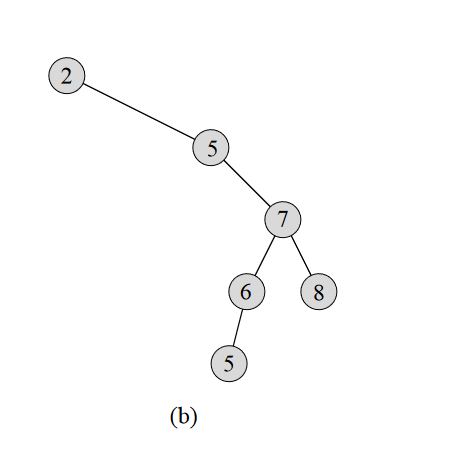
\includegraphics[width=8cm]{bst.PNG}
     \caption{Fig 12.1(b)}
     \label{fig:my_label}
 \end{figure}
\end{example}
\vspace{1em}
\begin{remark}
Nodes with no children are called leaves. Nodes which are not leaves are called internal nodes. Nodes with the same parent are called siblings. 
\end{remark}
\vspace{1em}
\textbf{Solution:} 
\textbf{Pre-order} $\langle 2,5,5,6,7,8\rangle$
\begin{definition}
\textbf{Preorder-Tree-Walk(x) } x (root), x's left subtree, and x's right subtree. \\
(Visit the root, traverse the left subtree, traverse the right subtree)
\begin{lstlisting}[escapeinside={(*}{*)}]
if x (*$\neq$*) NIL 
    print(x.key)
    Preorder-Tree-Walk(x.left) //Left subtree
    Preorder-Tree-Walk(x.right)
\end{lstlisting}
\end{definition}
\textbf{Post-order:} $\langle 5,6,8,7,5,2\rangle$
\begin{definition}
\textbf{Postorder-Tree-Walk: } x's left subtree, x's right subtree, and x (root).\\
(Traverse the left subtree, traverse the right subtree, visit the root)
\begin{lstlisting}[escapeinside={(*}{*)}]
if x (*$\neq$*) NIL
    Postorder-Tree-Walk(x.left) //Left subtree
    Postorder-Tree-Walk(x.right) //Right subtree
    print(x.key)
\end{lstlisting}
\end{definition}
\begin{remark}
Keys in a BST may or may not be distinct. Figure 4.1 has duplicate values. 
\end{remark}
\vspace{1em}
\begin{example}
A full binary tree of 7 nodes, find Inorder, Pre-order, Post-order 
\begin{figure}[h!]
    \centering
    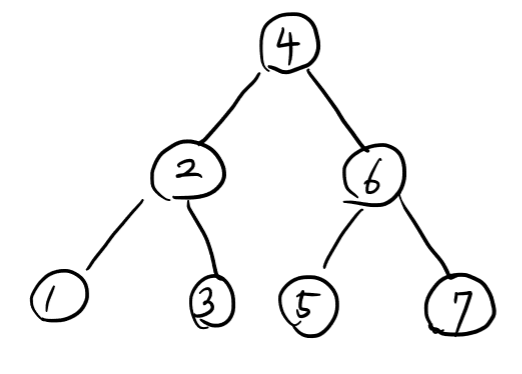
\includegraphics[width=8cm]{exnode7.PNG}
    \caption{Full Binary Tree}
    \label{fig:my_label}
\end{figure}
\end{example}
\vspace{1em}
\begin{remark}
A full binary tree is a binary tree in which each node has exactly zero or two children. \\
A complete binary tree is $\Theta(\log(n))$ in worst case.
\end{remark}
\vspace{1em}
\textbf{Solution:}
\begin{itemize}
    \item \textbf{Inorder} $\langle \color{red}1,2,3\color{black},4,\color{blue}5,6,7\color{black} \rangle$
    \begin{definition}
    \textbf{Inorder-Tree-Walk: } x's \color{red}left \color{black} subtree, x (root), and x's \color{blue}right \color{black}  subtree. \\
    (Traverse the left subtree, visit the root, traverse the right subtree)
\begin{lstlisting}[escapeinside={(*}{*)}]
    if x (*$\neq$*) NIL 
        Inorder-Tree-Walk(x.left)
        Inorder-Tree-Walk(x.right)
        print(x.key)
\end{lstlisting}
    \end{definition}
    \item \textbf{Pre-order} $\langle 4,\color{red}2,1,3\color{blue},6,5,7\color{black} \rangle$
    \item \textbf{Post-order} $\langle \color{red}1,3,2,\color{blue}5,7,6\color{black},4 \rangle$
\end{itemize}
\begin{remark}
The worst-case running time for most search-tree operations is proportional to the height of the tree.
\end{remark}
\vspace{1em} 
\subsection{Sequence of nodes} 
\begin{example}
Suppose that we have numbers between 1 and 1000 in a binary search tree, and we want to search for the number 363. Which of the following  sequences could not be a sequence of nodes examined? 
\end{example}
\vspace{1em}
\textbf{Consider the following}\\
\textbf{Binary-Search-Tree Property} 
\begin{definition}
For any node x in BST. 
\begin{itemize}
    \item If y is in left subtree of x, then y.key $\leq$ x.key 
    \item If y is in the right subtree of x, then y.key $\geq $ x.key
\end{itemize}
\end{definition}
\begin{enumerate}[label=(\alph*)]
    \item 2,252,401,398,330,344,397,363
    \item 924,220,911,244,898,258,362,363
    \color{red}
    \item 925,202,911,240,912,245,363\\
    \textbf{Does not meet BST property } Since $911 < 912$. BST in Figure 4.3\color{black}
    \item 2,399,387,219,266,382,381,278,363
    \item 935,278,347,621,299,392,358,363
\end{enumerate}
\vspace{1em}
Construct Binary Search Tree
\begin{enumerate}
    \item Make the first element the root (x)
    \item For the next element (y) 
    \begin{itemize}
        \item If value (y.key) is $\leq$ node.value (x.key)\\ Place left
        \item If value (y.key) is $>$ node.value (x.key)\\
        Place right 
        \item If the place is empty \\ 
        Place the node 
    \end{itemize}
\end{enumerate}
\begin{figure}[h!]
    \centering
    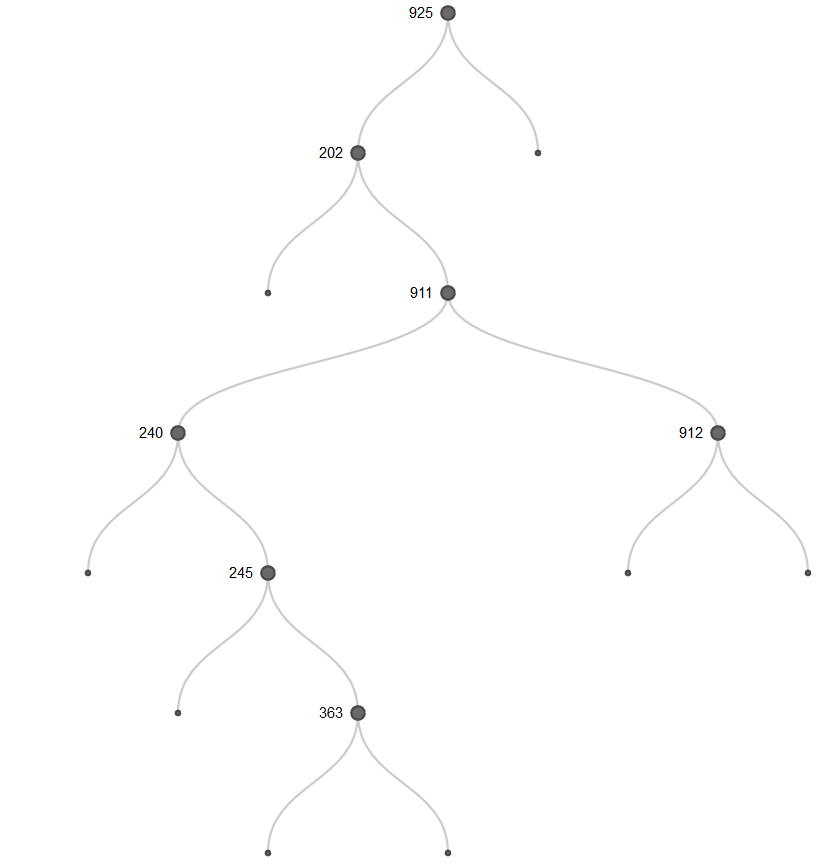
\includegraphics[width=90mm]{bstC.PNG}
    \caption{Part (c)}
    \label{fig:example_4_3}
\end{figure}
\begin{remark}
The sequence of nodes are valid if you can easily traverse through them to find a value. If the BST has a single path, then it is valid. 
\end{remark}
\subsection{Binary Search Tree Problem}
\vspace{1em}
\begin{example}
Consider the following binary search tree where nodes are labeled by alphabets. Here the keys are not shown in the picture; \textit{a,b,c,\dots} are node labels, not keys. Assume that all keys have distinct values. \\
\begin{figure}[h!]
    \centering
    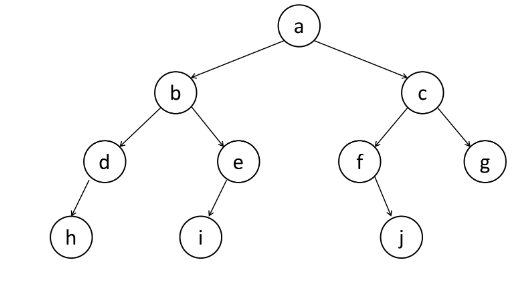
\includegraphics[width=90mm]{bst4.PNG}
    \caption{Example 3.4}
    \label{fig:my_label}
\end{figure}
\end{example}
\vspace{1em}
\begin{enumerate}[label=(\Alph*)]
    \item What is the node with the min key value? \\
    \begin{definition}
    \textbf{TREE-MINIMUM(x): } The min key is at the leftmost node. 
    \begin{lstlisting}
    while x.left != NIL
        x = x.left 
    return x
    \end{lstlisting}
    \end{definition}
    \textbf{Solution : } Node \textit{h} has the min key value.
    \item What is the node with the max key value? \\
    \begin{definition}
    \textbf{TREE-MAXIMUM(x): } The max key is at rightmost node.\\
    \begin{lstlisting}
    while x.right != NIL 
        x = x.right 
    return x
    \end{lstlisting}
    \end{definition}
    \textbf{Solution : } Node \textit{g} has the max key. 
    \begin{remark}
    Running time for TREE-MINIMUM and Tree-MAXIMUM is O(\textit{h}) where \textit{h} is the subtree's height. 
    \end{remark}
    \item What is the node with the upper median key value? 
    \begin{definition}
    
    \end{definition}
    \item What is the node with the lower median key value? 
    \item What is \textit{e}'s successor?
    \begin{definition}
    \textbf{Successor: } The successor of a node x is the node y such that y.key  is the smallest key greater than x.key
    \begin{lstlisting}
    if x.right != NIL
        return TREE-MINIMUM(x.right)
    y = x.p //(Parent of x) 
    while y != NIL and x == y.right 
        x = y
        y = y.p //(Parent of y) 
    return(y)
    \end{lstlisting}
    \end{definition}
    \textbf{Solution :} The successor is \textit{a}. 
    \begin{enumerate}
        \item \textbf{Lines 1-2: } Start at node label 
    \textit{e} (x), the right subtree of \textit{e} is NIL (x.right) therefore \textbf{line 2} does not execute.  
        \item \textbf{Line 3: } y is set to the parent of x (x.p)  which is node label \textit{b}
        \item \textbf{Lines 4: While Loop} Since y is \textit{b} it is not NIL and (y.right) is  x which is \textit{e}. 
        \item \textbf{Lines 5-6: Inside While} Set x equal to y which is \textit{b}, and y equal to parent of y which is  \textit{a}. 
        \item \textbf{Lines 4: While Loop} y is b and not NIL and (y.right) is x which is \textit{a}
        \item \textbf{Lines 5-6: Inside While} Set x equal to y which is \textit{b}, and y equal to the parent of y which is NIL (y.p).
        \item \textbf{Lines 7} While loop terminates. Returns y which node label \textbf{a} 
    \end{enumerate}
    \item What is \textit{i}'s successor?\\
    \textbf{Solution: } The successor is \textit{e}
    \begin{enumerate}
        \item \textbf{Lines 1-2:} Start at node label \textit{i}, the right subtree of \textit{i} is NIL (x.right) therefore \textbf{line 2} does not execute. 
        \item \textbf{Line 3:} y is set to the parent of x (x.p) which is node label \textit{e}
        \item \textbf{Line 4: While Loop} Since y is \textit{e} it is not NIL and (y.right) is NIL not x, the while loop does not execute \textbf{Lines 5-6}.
        \item \textbf{Line 7:} Returns y which is node label \textbf{e}.
    \end{enumerate}
    \item What is \textit{g}'s successor?\\
    \textbf{Solution: } The successor is \textit{a}
    \begin{enumerate}
        \item \textbf{Line 1-2:} Start at node label \textit{g} (x), the right subtree  is NIL (x.right) therefore \textbf{line 2} does not execute. 
        \item \textbf{Line 3:} y is set to the parent x (x.p) which is node label \textit{c} 
        \item \textbf{Line 4: While Loop} Since y is \textit{c} it is not NIL and (y.right) is x which is \textit{g} 
        \item \textbf{Line 5-6: Inside While } Set x equal to y which is \textbf{c}, and y equal to the parent of y which is \textit{a}. 
        \item \textbf{Line 4: While Loop} Since y is \textit{a} and (y.right) is x which is \textit{c}. 
        \item \textbf{Line 5-6: Inside While} Set x equal to y which is \textbf{a} and y equal to the parent of y which is \textbf{NIL}
        \item \textbf{Line 4: While Loop} Since y is NIL \textbf{Lines 5-6} do not execute. 
        \item \textbf{Line 7: } Returns y which is node label \textbf{a}.
    \end{enumerate}
    \item What is \textit{j}'s predecessor?\\
    \textbf{Solution: } The predecessor is \textit{c}
\end{enumerate}
\begin{remark}
The running time for \textbf{successor} and \textbf{predecessor} is $O(h)$
\end{remark}
\begin{example}
Consider the BST in the above problem. 
\end{example}
\begin{definition}
Find the minimum of right subtree, copy that value to the node that will be deleted, and delete the duplicate from the right subtree. \\
Find maximum in left subtree, copy that value to the node that will be deleted, and then delete the duplicate from the right subtree. 
\end{definition}
\begin{enumerate}[label=(\Alph*)]
    \item Delete node b and show the resulting BST\\
    \textbf{Solution: } Remove \textit{b} and replace with minimum in rights subtree. We find \textit{e} to be the minimum. 
    \begin{center}
    \tikzset{every tree node/.style={minimum width=2em,draw,circle},
         blank/.style={draw=none},
         edge from parent/.style=
         {draw,edge from parent path={(\tikzparentnode) -- (\tikzchildnode)}},
         level distance=1.5cm}
\begin{tikzpicture}
\Tree
[.$a$     
    [.$i$ 
        [.$d$
        \edge[]; \node[]{$h$};
        \edge[blank]; \node[blank]{};
        ]
        [.$e$
        \edge[blank]; \node[blank]{};
        \edge[blank]; \node[blank]{};
        ]
    ]
    [.$c$
        [.$f$
        \edge[blank]; \node[blank]{};
        \edge[]; \node[]{$j$};
        ]
        \edge[]; \node[]{$g$};
    ]
]
\end{tikzpicture}
\end{center}
    \item Continue to delete another node c and show the resulting BST.\\
\begin{center}
     \tikzset{every tree node/.style={minimum width=2em,draw,circle},
         blank/.style={draw=none},
         edge from parent/.style=
         {draw,edge from parent path={(\tikzparentnode) -- (\tikzchildnode)}},
         level distance=1.5cm}
\begin{tikzpicture}
\Tree
[.$a$     
    [.$i$ 
        [.$d$
        \edge[]; \node[]{$h$};
        \edge[blank]; \node[blank]{};
        ]
        [.$e$
        \edge[blank]; \node[blank]{};
        \edge[blank]; \node[blank]{};
        ]
    ]
    [.$g$
        [.$f$
        \edge[blank]; \node[blank]{};
        \edge[]; \node[]{$j$};
        ]
    ]
]
\end{tikzpicture}
\end{center}
    \item Continue to delete another node h and show the resulting BST. \\
\begin{center}
     \tikzset{every tree node/.style={minimum width=2em,draw,circle},
         blank/.style={draw=none},
         edge from parent/.style=
         {draw,edge from parent path={(\tikzparentnode) -- (\tikzchildnode)}},
         level distance=1.5cm}
\begin{tikzpicture}
\Tree
[.$a$     
    [.$i$ 
        [.$d$
        %\edge[]; \node[]{$h$};
        \edge[blank]; \node[blank]{};
        ]
        [.$e$
        \edge[blank]; \node[blank]{};
        \edge[blank]; \node[blank]{};
        ]
    ]
    [.$g$
        [.$f$
        \edge[blank]; \node[blank]{};
        \edge[]; \node[]{$j$};
        ]
    ]
]
\end{tikzpicture}
\end{center}
\end{enumerate}
\begin{remark}
When leaf nodes are deleted the BST property is maintained. Leaf nodes do not have right or left children. When deleting an internal node that has only one child remove internal node and link its parent to the child.  
\end{remark}
\section{Advanced}
\section{Sources and Resources}
In order to fully understand the concepts here. Consider the following items. \\
\href{https://www.cs.rochester.edu/~gildea/csc282/slides/C12-bst.pdf}{https://www.cs.rochester.edu/~gildea/csc282/slides/C12-bst.pdf}
\chapter{Elementary Graph Algorithms} 
\section{Basic}
\vspace{1em}
\subsection{Properties of BFS and DFS}
\vspace{1em}
\begin{example}
To implement BFS, what data structure do you use? What about DFS (if we use no recursion)?
\end{example}
\begin{definition}
\textbf{Breadth First Search (BFS):} 
\begin{enumerate}
    \item \textbf{INPUT:} Graph $G = (V,E)$ and a source $s$. 
    \item \textbf{OUTPUT:} A tree (Breadth First Tree) consisting of vertices reachable from $s$ encoding distance from source vertex $s$
    \begin{itemize}
    \item The vertices that are reachable from $s$
    \item The shortest distance from $s$ to each reachable vertex
    \item A shortest paths tree that allows reporting the shortest path from $s$ to a reachable vertex.
    \end{itemize}
    \item Works on Direct and Undirected graphs
      \item Time Complexity is $\Theta(V + E)$
    \item Uses a queue (FIFO) data structure. 
\end{enumerate}
\end{definition}
\begin{definition}
\textbf{Depth First Search (DFS): } 
\begin{enumerate}
    \item \textbf{INPUT:} Graph $G = (V,E)$ and no source. 
    \item \textbf{OUTPUT:}
    \begin{itemize}
        \item  $\pi$ to record predecessors (to encode the resulting DFF)
        \item two timestamps on each vertex $v$
    \end{itemize}
    \item Time complexity is $\Theta(V + E)$ if g is represented using \textbf{adjency lists} 
    \item Information about structure of graph. 
\end{enumerate}
\end{definition}
\textbf{Solution: } 
\begin{enumerate}
    \item To implement Breadth First Search (BFS) we use a queue data structure. First In First Out (FIFO)
    \item For Depth First Search (DFS) we use a stack. Last In First Out (LILO)
\end{enumerate}
\subsection{Undirected and Directed Graph}
\vspace{1em}
\begin{example}
We're given a directed graph G, along with a pair of vertices, \textit{u} and \textit{v}. We would like to know if there is a path from \textit{u} to \textit{v}. 
What algorithm would you like to use?
\end{example}
\begin{definition}
\textbf{Graph:} $G = (V,E)$. V is set of vertices. E is set of edges. 
\end{definition}
\begin{definition}
\textbf{Undirected Graph:} Edges are unordered pairs. 
\begin{itemize}
    \item Edges $(u,v)$ and $(v,u)$ are the same. 
    \item Edges go from one vertex to another. 
    \item No self loop. A \textit{self-loop} is an edge that connects a vertex to itself. (v,v) $\not \in E$ 
\end{itemize}
\end{definition}
\begin{figure}[h!]
    \centering
    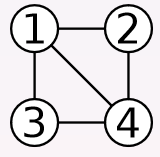
\includegraphics{UG.PNG}
    \caption{Undirected Graph}
    \label{fig:my_label}
\end{figure}
\begin{definition}
\textbf{Directed Graph: } Edges are ordered pairs. 
\begin{itemize}
    \item Edges $(u,v)$ and $(v,u)$ are different. 
    \item \textit{u} is called tail, and \textit{v} is the head. 
\end{itemize}
\end{definition}
\begin{figure}[h!]
    \centering
    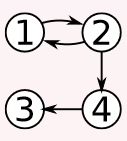
\includegraphics{Pictures/dg.PNG}
    \caption{Directed Graph}
    \label{fig:my_label}
\end{figure}
\textbf{Solution:} The algorithm Breadth First Search (BFS). 
 
\subsection{Definition of Breadth First Tree (BFT)}
\vspace{1em}
\begin{example}
What is the definition of BFT (breadth first tree)? \\Suppose the graph consideration is undirected. 
Could there be an edge between two vertices whose depths differ by more than one? 
\end{example}
\begin{definition}
\textbf{Breadth First Tree} 
\end{definition}
\subsection{BFS and DFS problem}
\vspace{1em}
\begin{example}
Consider the following directed graph. 
\begin{center}
\begin{figure}[H]
    \centering
    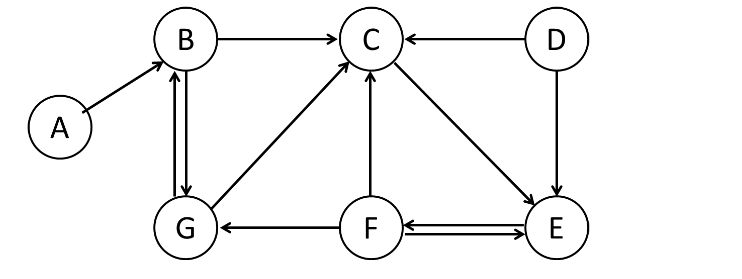
\includegraphics{disc22_04.PNG}
    \caption{(a) through (h)}
    \label{}
\end{figure}
\end{center}
\end{example}
\begin{enumerate}[label=(\alph*)]
    \item Draw the adjacency-list representation of G, with each list sorted in increasing alphabetical order.
    \vspace{1em}
    \begin{definition}
    \textbf{Adjacency-list} Represents the graph $G = (V,E)$ as an array of linked list. The index of the array represents a vertex and each element in its linked list represents the other vertices that form an edge with the vertex.
    \end{definition}
    
    \begin{enumerate}[label=(\arabic*)]
        \item Each vertex in the graph is placed in a box in the left hand column
        \item Each adjacent vertex is shown as a node in the list to its right.
        %\begin{itemize}
        %\item Vertex \textbf{A} has one edge. 
        %\item Vertex \textbf{B} has two edges.
        %\item Vertex \textbf{C} has one edge.
        %\item Vertex \textbf{D} has two edges.
    %\end{itemize}
        \item The arrows indicate the next node in the list.
    \end{enumerate}
    \begin{remark}
    Generally the order of the vertices in an adjacency list do not matter unless specified.
    \end{remark}
    \textbf{Solution:}
    \begin{figure}[H]
        \centering
        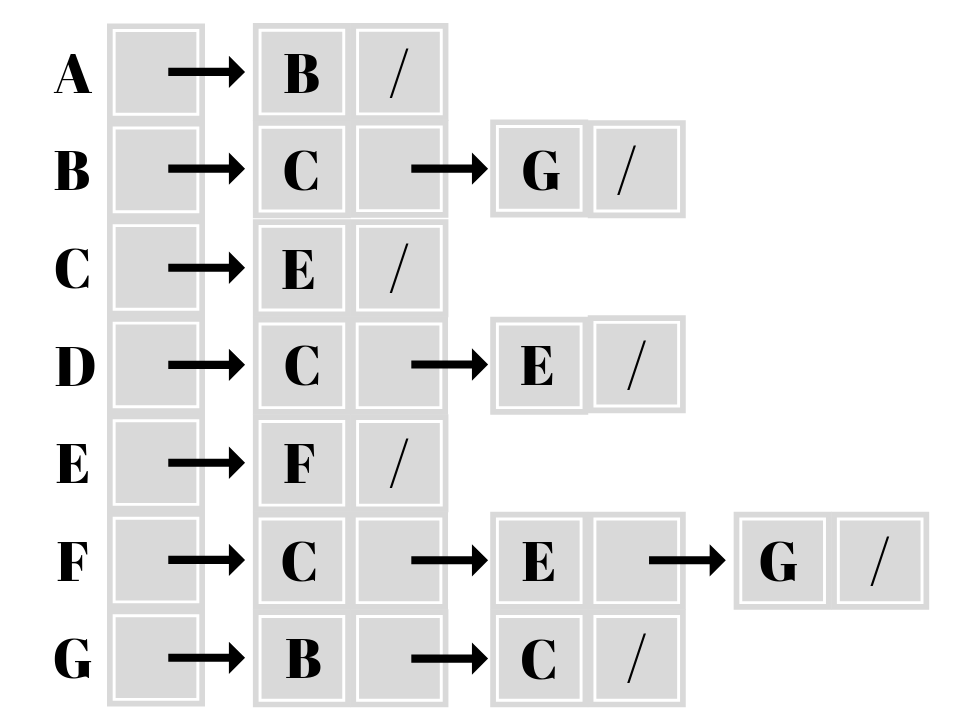
\includegraphics[width=140mm]{Pictures/al1.png}
        \caption{(a)}
        \label{fig:my_label}
    \end{figure}
    \item Give the adjacency matrix of G. 
    \vspace{1em}
    \begin{definition}
    \textbf{Adjacency Matrix} of a graph $G = (V,E)$ is represented by a $|V|\times|V|$ matrix, $A = (a_{ij})$ where $a_{i,j} = 1$ if $(i,j) \in E$ and 0 otherwise. 
    \end{definition}
   \begin{enumerate}[label=(\arabic*)]
       \item There are 7 vertices (|V|). The matrix should be $7\times7$
       \item If there exists and edge between two vertices then $a_{ij}$ is \textit{True (1)} otherwise \textit{False (0)} 
   \end{enumerate}
   \begin{center}
  \lettrine[findent=2pt]{\textbf{A = }}{ } 
   \begin{tabular}{c|c c c c c c c}
       & A & B & C & D & E & F & G \\
      \hline 
    A & 0 & 1 & 0 & 0 & 0 & 0 & 0 \\
    B & 0 & 0 & 1 & 0 & 0 & 0 & 1\\
    C & 0 & 0 & 0 & 0 & 1 & 0 & 0\\
    D & 0 & 0 & 1 & 0 & 1 & 0 & 0 \\
    E & 0 & 0 & 0 & 0 & 0 & 1 & 0\\
    F & 0 & 0 & 1 & 0 & 1 & 0 & 1\\
    G & 0 & 1 & 1 & 0 & 0 & 0 & 0\\
   \end{tabular}
   \end{center}
   \item Draw the graph, the adjacency-list representation (with each list sorted in increasing alphabetical order), and the adjacency matrix for the transpose graph $G^T$.
   \begin{definition}
   \textbf{Transpose of Graph: } Reverse the order of edges. \\
   $(u,v) \rightarrow (v,u)$ and $(v,u) \rightarrow (u,v)$ where $(u,v) \in E$. 
   \end{definition}
   \begin{itemize}
       \item Find the transpose $G^T$ 
       \begin{figure}[H]
       \centering
       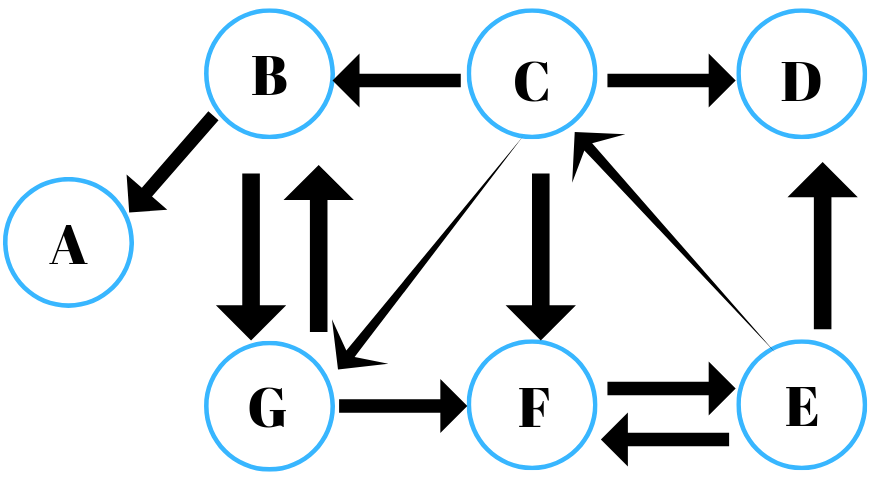
\includegraphics[width=100mm]{Pictures/gtranspose4_1.png}
       \caption{(c) $G^T$}
       \label{fig:my_label}
   \end{figure}
       \item Draw adjacency-list representation. 
       \begin{figure}[H]
           \centering
           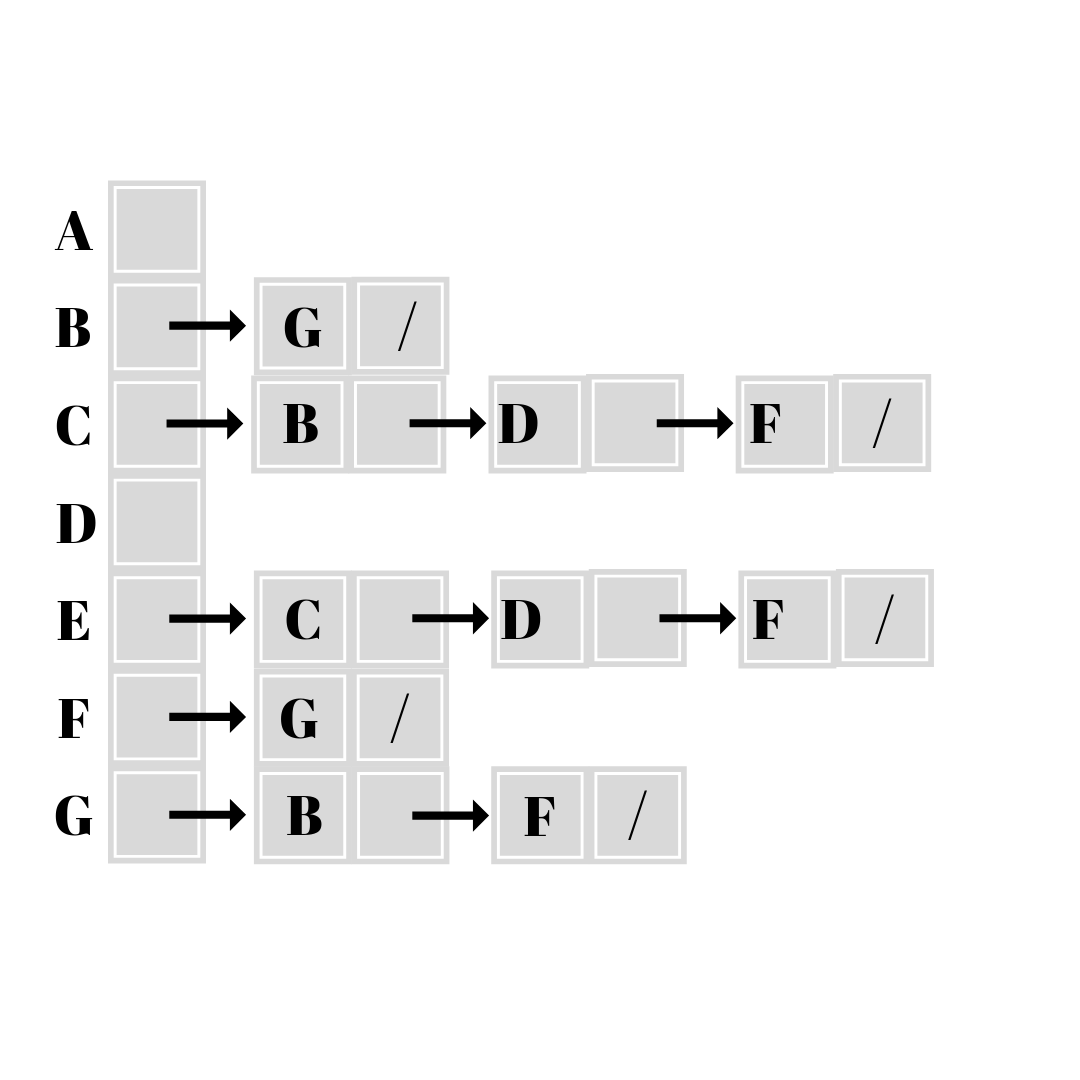
\includegraphics[width=140mm]{Pictures/alr_b.png}
           \caption{(c) Adjacency-list}
           \label{fig:my_label}
       \end{figure}
       \item Give adjacency matrix.
   \end{itemize}
   \item Do depth-first search in G, considering vertices in increasing alphabetical order. Show the final result, with vertices labeled with their starting and finishing times, and edges labeled with their type (T/B/F/C). 
   \item Based on your results, proceed to to run the algorithm to find the strongly connected components of G (show the result of the DFS in $G^T$, with vertices labeled with their starting and finishing times. 
   \item Draw the component graph $G^{SCC}$ of G
   \item Find a topological sort of $G^{SCC}$ using the following algorithms. (label each vertex with its DFS finishing time)
   \item Run BFS with B as a starting vertex. Show the tree edges produced by the BFS along with v.d of each vertex v. You must draw the current tree edges in each itration together with the queue status. More precisely, run BFS with B starting point assuming that each adjacency list is sorted in increasing alphabetical order. 
\end{enumerate}
\subsection{DFF }
\begin{example}
If \textit{u} is reachable from \textit{v, u} muse be a descendant of \textit{v} in any DFF. 
\end{example}
\section{Intermediate}
\section{Advanced} 
\chapter{Minimum Spanning Trees}
\section{Basic}
\subsection{Terminology}
\begin{example}
What is the definition of a Tree. 
\end{example}
\textbf{Solution:} 
A connected graph with no cycles.
\vspace{1em}
\begin{example}
If a tree \textbf{T} has n vertices, then \textbf{T} must have $n - 1$ edges? 
\end{example}
\begin{figure}[H]
    \centering
    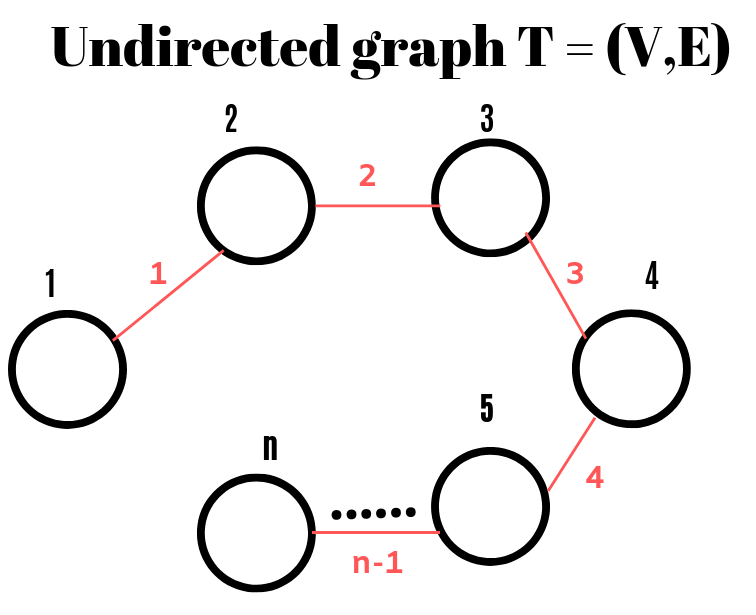
\includegraphics[width=100mm]{Pictures/treeT.png}
    \caption{Conneced  \textbf{T}}
    \label{fig:my_label}
\end{figure}
\textbf{Solution:} \textit{True}. A tree does not have cycles. A tree is an undirected graph in which any two vertices are connected by exactly one path.
\begin{remark}
\textbf{TRUE:} If a graph \textbf{G} = $(V,E)$ has |V| edges or more, then it must have a cycle. 
\end{remark}
\vspace{1em}
\begin{example}
Consider the pseudocode of \textbf{GENERIC-MST(G,w)}. Where the \textbf{Input:} Undirected graph $G = (V,E)$ and weight/cost $w(u,v)$ for every edge $(u,v)\in E$. What is the output? 
\end{example}
\textbf{GENERIC-MST(G,w)}
\begin{lstlisting}[escapeinside={(*}{*)}]
A = (*$\emptyset$*)
(*\textbf{While}*) A does not form a spanning tree
    find and edge (*$(u,v)$*) that is safe for A 
    (*$A = A \cup {(u,v)}$*)
return(A)
\end{lstlisting}
\begin{definition}
\textbf{Spanning Tree:} A tree that connects all vertices of $G = (V,E)$
\end{definition}
\begin{definition}
\textbf{Minimum Spanning Tree:} A spanning tree denoted \textbf{T} whose total edge weight is minimized. 
\end{definition}
\textbf{Solution:} A minimum spanning tree $T \subseteq E$
\begin{remark}
To find the \textbf{Spanning Tree} of a graph $G = (V,E)$ the vertices must be connected. 
\end{remark}
\vspace{1em}
\begin{example}
What is the definition of safe edges (assuming that edges have all distinct weights)? The lecture slides use a definition that is different from the textbook. Use the definition in the lecture slides, which is simpler. 
\end{example}
\textbf{Solution:} 
\chapter{Single-Source Shortest Paths}
\section*{Basic}
\vspace{1em}
\subsection{Optimality of subpaths}
\begin{example}
Explain why the following lemma is true. \\
\begin{lemma}
\textbf{Optimality of subpaths:} If $P = \langle v_0, v_1, \dots, v_k\rangle$ is a shortest path from $v_0$ to $v_k$, then for any $0 \leq i \leq j \leq k$, $\langle v_i, v_{i + 1}, \dots, v_{j}$ is a shortest path from $v_i$ to $v_j$. In other words, subpaths of shortest subproblems are also shortest paths.
\end{lemma}
\end{example}
\textbf{Solution:} One could get a "better" shortest path from $v_0$ to $v_k$ by replacing $\langle v_i, v_{i+1}, \dots, v_j$ with a better path from $v_i$ to $v_j$
\subsection{Bellman-Ford Algorithm}
\begin{example}
The Bellman Ford algorithm repeats relaxing the entire set of edges $|V| - 1$ times. Each iteration edges can be relaxed in an arbitrary order. Consider the following chain graph. The source vertex is \textit{s}.
\begin{figure}[H]
    \centering
    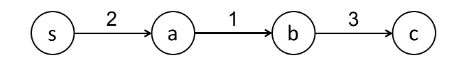
\includegraphics{Pictures/bfaChainG.PNG}
    %\caption{Chain Graph}
    \label{fig:my_label}
\end{figure}
Find the values of $s.d, a.d, b.d$ and $c.d$ after exactly one iteration, i.e. just after you relax all edges for $i = 1$, when edges are considered in each of the following orders? 
\begin{enumerate}[label=(\alph*)]
    \item (s,a), (a,b), (b,c).
    \item (b,c), (a,b), (s,a).
\end{enumerate}
\end{example}

%----------------------------------------------------------------------------------------
%	BIBLIOGRAPHY
%----------------------------------------------------------------------------------------


\begin{thebibliography}{9}
\bibitem{cormen} 
Thomas H. Cormen, Charles E. Leiserson, Ronald L. Rives, and Clifford Stein. 
\textit{Introdudction to Algorithms}. 
MIT, 2009.
 
\bibitem{SungjinWebsite} 
Sunjin: CSE 100 Algorithm Design and Analysis,
\\\texttt{http://faculty.ucmerced.edu/sim3/}

\bibitem{MiguelWebsite} 
Carreira-Perpiñan: CSE 100 Algorithm Design and Analysis,
\\\texttt{http://faculty.ucmerced.edu/mcarreira-perpinan/}

\end{thebibliography}


%----------------------------------------------------------------------------------------
\end{document}
